\documentclass{article}

\usepackage[T1]{fontenc}
\usepackage[utf8]{inputenc}
\usepackage{graphicx}
\usepackage{hyperref}
\usepackage{lmodern}
\usepackage{amssymb,amsfonts,amsmath,amsthm}
\usepackage{listings}
\usepackage{enumerate}
\usepackage{amssymb}
\usepackage{amsfonts}
\usepackage{multicol}
\usepackage{float}

\usepackage[margin=60pt]{geometry}

\author{Thibault Latrille, Laurent Duret, Nicolas Lartillot}
\title{The red queen dynamic in the kingdom of recombination.}  

\sloppy 

\begin{document}

\maketitle 

\newcommand{\avg}[1]{\left< #1 \right>} % for average
\newcommand{\Ne}{N_\mathrm{e}}
\newcommand{\Rp}{\theta}
\newcommand{\R}{R}
\newcommand{\Rt}{\R_{t}}
\newcommand{\D}{D}
\newcommand{\Dt}{\D_{t}}
\newcommand{\V}{V}
\newcommand{\Vt}{\V_{t}}
\newcommand{\T}{T}
\newcommand{\Rmin}{{\R_{\infty}}}
\newcommand{\dd}{\mathrm{d}}


\newcommand{\Lr}{L}
\newcommand{\Lmin}{\Lr_{\infty}}
\newcommand{\Lmina}{\alpha}
\newcommand{\Lminb}{\beta}
\newcommand{\Lra}{\gamma}
\newcommand{\Lrb}{\delta}
%\tableofcontents             

\section*{Abstract}
In humans and many other species, recombination events cluster in narrow hotspots distributed across the genome, whose location is determined by the Zing-finger protein PRDM9. Surprisingly, hotspots are not shared between human and chimpanzee, suggesting that hotspots are short-lived. To explain this fast evolutionary dynamics of recombination landscapes, an intra-genomic Red-Queen model, based on the interplay between two antagonistic forces, has been proposed. On the one hand, biased gene conversion, mediated by double-strand breaks, results in a rapid extinction of hotspots in the population. On the other hand, the resulting genome-wide depletion of recombination induces strong positive selection favoring new Prdm9 alleles recognizing new sequence motifs across the genome, thereby restoring normal levels of recombination. Thus far, however, this Red-Queen scenario has not been formalized as a quantitative model.

Here, we propose a detailed population-genetic model of the Red-Queen dynamic of recombination. This model was implemented as a Wright-Fisher simulator, allowing exploration of the behaviour of the model (in terms of the implied mean equilibrium recombination rate, diversity at the PRDM9 locus, or turnover rate) as a function of the parameters (effective population size, mutation rate). In a second step, analytical results, based on self-consistent mean-field approximations, were derived. These analytical results reproduce the scaling relations observed in the simulations, offering key insights about the detailed population-genetic mechanisms of the Red-Queen model. These insights and scaling relations can now be tested against empirical data currently available in mammals.

\section*{Introduction}
PRDM9 is a meiosis-specific histone methyltransferase with a tandem-repeat zinc finger (ZnF) domain encoded by a mini-satellite-like sequence. The ZnF domain is polymorphic in repeat number and type, and appears to be directly responsible for activating recombination hotspots by binding to hotspot-associated sequence motifs in both humans and mice.

Hotspots evolve rapidly, as shown by the totally different fine-scale recombination landscapes of humans and chimpanzees.
Turnover might be driven by the tendency of hotspots to self-destruct through the systematic over-transmission of variants within hotspots that down-regulate recombination initiation, leading to hotspot depletion and consequent 
selection in favour of PRDM9 variants that activate new sets of hotspots.

We are interested in a mathematical modelling of the turnover of PRDM9 variants and the associated recombination hotspots.

\section*{Materials and methods}

\subsection*{Population genetic model}

We built a Wright-Fisher population genetic model.
The population is composed of $\Ne$ diploid individuals, kept constant over time.

\subsection*{PRDM9 mutation}

The locus PRDM9 mutates at constant rate $u$ per generation per locus and each new variant binds a new sets of sequence targets. Thus $u$ can be understood as a functional mutation rate, with each mutation producing a new PRDM9 variant with new hotspots.

At each generation, $K_{t}$ is the number of PRDM9 alleles in the population. $\forall i \in \{ 1, \, \dots, \, K_{t} \}$, $n_{i,t}$ is the number of $i^{th}$ PRDM9 allele in the population. Consequently, $x_{i,t} = n_{i,t} / 2 \Ne$ is the frequency of the $i^{th}$ PRDM9 allele.

\subsection*{Erosion of the hotspots}

Whenever a new allele appears it has access to a complete set of functional hotspots. Thus the activity is maximal, and progressively hotspots are eroded by dBGC leading to a decreasing activity. 

For each allele $i$,  $\Rp _{i,t}$ is the activity at time $t$. We model the evolution of $\Rp _{i,t}$ implicitly.

\begin{equation}
\left\{
      \begin{aligned}
 & \dfrac{\dd \Rp _{i,t+1} }{\dd t} =  - \rho \Rp _{i,t} x_{i,t}, \;
 \forall i \in \{ 1, \, \dots, \, K \} \\
 & \rho = 4 \Ne v r _0
      \end{aligned}
\right. 
\end{equation}


Arguments behind this phenomenological model: 

- At any given time, most hotspots associated with a given PRDM9 allele are either fully active, or fully inactive. Meaning a minor fraction of hotspots are in polymorphic state.

- $\Rp _{i,t}$ can be thought as the proportion of active hotspots.

- rate of substitution from active to inactive hotspots is the mutation rate ($2 \Ne v$) time the fixation probability of mutant hotspots ($2 r_0$)

\subsection*{Selection of PRDM9}

For each allele, $\Rp _{i,t}$ is the overall activity of the sequence targets, with $\Rp _{i,t}=1$ meaning no activity and $\Rp _{i,t}=0$ meaning totally eroded.

$\overline{\omega_{i,t}}$ is fitness of this allele. At the population level, $\overline{\omega}=\sum_{i} x_{i,t} \overline{\omega_{i,t}}$ is the mean fitness.

We propose $\overline{\omega_{i,t}}=\sum_{j \in K_{t}} x_{j,t} f \left( \dfrac{\Rp _{i,t} + \Rp _{j,t}}{2} \right)$, for any function $f\colon [0,1] \rightarrow \mathbb{R}^+$. Meaning the fitness of allele $i$ is the sum over the probabilities that the second allele is $j$ (diploid individuals) time a function of the mean activity between allele $i$ and $j$. Thus we assume linear (additive) effect between alleles.

\subsection*{Overall simulation cycle} 

For each new generation, the simulation is decomposed in three steps, computed in the following order: \\

1. Mutation and creation of new alleles of PRDM9 

Per locus, PRDM9 mutates at constant rate $u$, and we have $2 \Ne$ loci in the population. Thus the number of new alleles is Poisson distributed with mean $2 \Ne u$. The new alleles are introduced in the population at a frequency $1 / 2 \Ne$

\begin{equation}
  K_{t+1} - K_{t} \sim \operatorname{Pois} \left(2 \Ne u \right)
\end{equation}

2. Erosion of the recombination hotspots 

The number of new mutation occurring in the population at the targets is $ \Ne v$, each of them are driven by a selection coefficient $ r _0  x_{i,t}$, where $x_{i,t}$ is the probability of activation by the allele $i$.
Since the activity is proportional to the targets being not eroded, we model the activity as an exponential decay.

\begin{align}
 \Rp _{i,t+1} &=  \Rp _{i,t}\operatorname{exp} \left( - \rho x_{i,t} \right), \;
 \forall i \in \{ 1, \, \dots, \, K \}
\end{align}

3. Drift and selection

The new generation of $2 \Ne$ PRDM9 alleles is drawn from a multinomial distribution, generating a drift. The probability of drawing allele $i$ is equal to it's frequency $x_{i,t}$ time it's relative fitness  $\dfrac{\overline{\omega_{i,t}}}{\overline{\omega}}$. The probabilities sum to $1$ by definition of $\overline{\omega}$.

\begin{align}
  & \left(
  n_{1, t+1}, \,
  \dots, \,
  n_{i,t+1}, \,
  \dots, \,
  n_{K_{t+1}}
  \right)  \, \sim \operatorname{Multinomial} \left(2 \Ne, \,
  \dfrac{x_{1,t}  \overline{\omega_{1,t}}}{\overline{\omega}}, \,
  \dots, \,
  \dfrac{x_{i,t}  \overline{\omega_{i,t}}}{\overline{\omega}}, \,
  \dots, \,
  \dfrac{x_{K_{t}} \overline{\omega_{K_{t}}}}{\overline{\omega}}  \right)
\end{align}


The model was implemented numerically by Monte Carlo simulations in Python, the code is hosted at \url{https://github.com/ThibaultLatrille/RedQueen}.

\subsection*{Summary statistics} 

To explore the behaviour of the Wright-Fisher model as a function of the parameters, one need to have summary statistics that gives insight on the dynamic of the red-queen. We focus on four measures, 
the diversity at PRDM9 locus, the mean recombination rate, 
Summary statistics are computed when the simulation reaches the limit cycle (attractor) of the red-queen. In out simulations are taken as the mean over many cycles (100 cycles). 

1. Diversity of PRDM9

Diversity can be defined in several ways; for example the richness $K_{t}$, defined above as the number of alleles, is a measure of PRDM9 diversity.
One shortcoming for $K_{t}$ is that it gives equal weight to all alleles, regardless of their frequencies in the population.
Thus as a measure of diversity we focused on the reciprocal of Simpson's index $D$ \cite{Hill1973}, which do obey the replication principle.
The replication principle states that if we have N equally large, equally diverse groups of PRDM9 alleles with no alleles in common, the diversity of the pooled groups must be N times the diversity of a single group.
$\Dt$ equals $K_{t}$ if all the alleles have equal weights and is close to $1$ if an allele has appreciable abundance.

\begin{align}
     \D &= \avg{\Dt} = \avg{\dfrac{1}{\sum_{i \in K_{t}} x_{i,t}^2}} 
\end{align}

2. Mean relative recombination rate

$\Rp _{i,t}$ is the relative recombination rate of the $i^{th}$ PRDM9 allele. Thus at the population level, the recombination rate is obtained by taking the weighted mean.

\begin{align}
    \R &= \avg{\Rt} = \avg{\sum_{i \in K_{t}} x_{i,t} \Rp _{i,t}} 
\end{align}

3. Landscape of the hotspots

Considering the number of hotspots in the genome is small compare to the 

\begin{align}
     \V &= \avg{\Vt} = \avg{\sum_{i \in K_{t}} x_{i,t}^2 \Rp _{i,t}} 
\end{align}

4. Turn-over of PRDM9

The turn-over is defined as the decorrelation time of the relative cross-homozygosity.
It is such that 

\begin{align}
   \T = \avg{\dfrac{\sum_{i \in K_{t}} x_{i,t} x_{i,t+T}}{\sum_{i \in K_{t}} x_{i,t} x_{i,t}}  }  =  \dfrac{1}{2}
\end{align}

\section*{Results}
\subsection*{Simulation results} 

Brief reminder about model. Wright-Fisher with mutation and selection. Only PRMD9 locus; evolutionary dynamics at PRDM9 target loci (hotspots) is implicit.

Figure scaling relations !

Equilibrium recombination rate is suboptimal ($\R < 1)$. Equivalently there is a recombination load associated to the red-queen.

Mean equilibrium recombination rate ($\R$) is constant as a function of $\Ne$, increases with $u$ and decreases with $v$.

Plotting the PRDM9 diversity ($\D$) as a function of $\Ne$ and $u$ reveals two distinct regimes: succession regime and polymorphic regime, essentially depending on the scaled mutation rate ($\Ne u$) at the PRDM9 locus. For low scaled mutation rates, one PRDM9 alleles at a time. For high scaled mutation rate, multiple alleles segregate in the population: in the regime $\D$ is roughly proportional to $\Ne u$.

In succession regime: turn-over time ($\T$) decreases with $\Ne$, reaching a maximum at the transition between the two regimes. Then, turn-over time remains constant.

Conversely, variance of recombination landscape ($\V$) first remains constant as a function of $\Ne$ in succession regime, then starts to decrease with $\Ne$ in polymorphic regime.

Thus as a function of $\Ne$, red-queen first unfolds as a succession of PRDM9 alleles, one at a time: recombination is then always concentrated on one single set of hotspots (corresponding to current dominant PRDM9 allele). As $\Ne$ increases, red-queen accelerates, up to a point where successive waves of erosion-invasion start to overlap, such that multiple PRDM9 alleles start to coexist in the population. In this regime, turn-over time now remains constant, as a function of $\Ne$. On the other hand, diversity at the PRDM9 locus increases, such that recombination is progressively spread over an increasing number of weaker hot-spots.

\subsection*{Analytical approximations in succession regime} 

In a succession regime, PRDM9 alleles don't co-segregate. There is only one allele at a time, and it's recombination rate ( $\Rp_{t}$) is decreasing proportionally to itself (biased gene conversion) at a rate $\rho = 4 \Ne v r_0$. Thus $\Rp_{t}$ follow an exponential decrease.

\begin{align} 
   \dfrac{\dd \Rp_{t}}{\dd t}  &=  - \rho \Rp_{t} \\
        \Rightarrow \Rp_{t} &= \operatorname{e}^{-\rho t}
\end{align}

The recombination rate  ($\Rp_{t}$) decreases up to point where a new PRDM9 allele invade the population. We call $\tau$ the mean time between two invasion of alleles. Thus when new alleles are invading, the resident alleles recombination rate are $\Rmin$ and we have :
\begin{equation}
   \Rmin =  \operatorname{e}^{-\rho \tau}
\end{equation}

Moreover the mean recombination rate $\R$ of alleles between there invasion and extinctions can be derived explicitly and leads to a relation between $\R$ and $\Rmin$: 

\begin{align} 
	R &= \avg{\Rp_{t}} \\
	\Rightarrow 0 &=  1-\Rmin  + \R  \operatorname{log}(\Rmin ) 
\end{align}

Using population genetic arguments, we can derive the substitution rate between two consecutive allele $\lambda_t$. This is the probability of fixation of a new allele that mutates at rate $u$ in a population of size $\Ne$ with selection coefficient $ 2 s(\Rp_{t}) $. The selection coefficient is derived in appendix after linearisation and leads to the equation : 

\begin{equation}
 \lambda_t = 2 \Ne u 2 s(\Rp_{t}) = \mu \dfrac{f'(\Rp_{t})}{f(\Rp_{t} )} (1 - \Rp_{t} ) 
\end{equation}
, with $\mu = 2 \Ne u $ 
And the mean time between two invasion of alleles ($\tau$) can be also derived as $\avg{\lambda_t^{-1}}$  .

\begin{equation}
\tau = \avg{\dfrac{1}{\lambda_t}} = \dfrac{1}{ \mu }\avg{\dfrac{f(\Rp_{t} )}{f'(\Rp_{t})(1 - \Rp_{t} )}}  = \dfrac{f(\R )}{ \mu f'(\R)(1 - \R) }
\end{equation}

And thus we get a self-consistent equation on $\R$ 
\begin{align} 
	& \dfrac{f'(\R )}{f(\R )} \dfrac{(1- \R )(1- \Rmin )}{\R } = \dfrac{\rho }{ \mu} = \dfrac{2 v r_0}{u} \\
	\Rightarrow  & \R= g\left(\dfrac{2 v r_0}{ u}\right)
\end{align}

Where $g$ is a strictly decreasing function cannot be solved explicitly but can be approximated (see section small load approximation). 
It is important to note that $\R$ is the independent if the population size $\Ne$, as our simulation was suggesting.

In the succession regime, the diversity at the PRDM9 locus $\D$ is simply equal $1$ since there is only one allele.
\begin{equation}
  \D = 1
\end{equation}

In the succession regime, the landscape of hotspots is the mean recombination rate ($\R$)
\begin{equation}
  \V = \R
\end{equation}

And finally, we get the turn-over time $\T$ 
\begin{equation}
  \T =  \tau = \dfrac{1 - \Rmin }{\rho \R }
\end{equation}

\subsection*{Analytical approximations in polymorphic regime}

By discarding the drift and linearising the activity, we derived a close set of differential equations for the frequencies of PRDM9 alleles ($x_{i,t}$) and there associated recombination rate ($\Rp_{i,t}$). 

\begin{equation}
\left\{
      \begin{aligned}
          \dfrac{\dd x_{i,t}}{\dd t} &= \dfrac{f'(\Rt )}{2 f(\Rt )} \left( \Rp_{i,t}  - \Rt  \right) x_{i,t}, \;
             \forall i \in \{ 1, \, \dots, \, K_{t} \} \\
        \dfrac{\dd \Rp_{i,t}}{\dd t} &= 
        - \rho x_{i,t} \Rp_{i,t}, \;
             \forall i \in \{ 1, \, \dots, \, K_{t} \} \\
             \Rt &= \sum_{i \in K_{t}} x_{i,t} \Rp _{i,t} 
      \end{aligned}
\right. 
\end{equation}

Under the assumption of many alleles co-segregating in the population and under a mean field approximation, then $\Rt=\R$ is independent of the trajectory followed by a single allele. This leads to a decoupling of the above system of equation, and we can study the trajectory of a single allele with frequency $x_{t}$ and relative recombination rate $\Rp _{t}$.
\begin{equation}
\left\{
      \begin{aligned}
          \dfrac{\dd x_{t}}{\dd t} &= \dfrac{f'(\R )}{2 f(\R )} \left( \Rp_{t}  - \R \right) x_{t} \\
        \dfrac{\dd \Rp_{t}}{\dd t} &= 
        - \rho x_{t} \Rp_{t} \\
      \end{aligned}
\right.
\end{equation}
Show plot and describe overall structure.

System of equations is not analytically solvable as a function of $t$. On the other hand, $\Rp_{t}$ is monotonic, and $x$ can be analytically expressed as a function of $\Rp_{t}$
\begin{equation}
x(\Rp_{t} ) =\dfrac{f'(\R)}{2 \rho f(\R )} (1- \Rp_{t}  + \R  \operatorname{log}(\Rp_{t} )) + x_{\mathrm{initial}}
\end{equation}

Since $x_{\mathrm{initial}} = 1 / \Ne \simeq 0$, we get an equation on $\R$ and $\Rmin$ when $x$ goes to zero.

\begin{align}
 	0 &=  x(\Rmin) \\
   \Rightarrow 0 &\simeq  1-\Rmin  + \R  \operatorname{log}(\Rmin ) 
\end{align}

Surprisingly, this is the same equation as in succession regime.

So far we considered $\R$ as an external parameter for a focal allele, but if every allele has the same trajectory, but with different arrival time, they all contribute back to $\R$. Thus we get a self-consistent estimation for  $\R$ using a tilling argument (see figure x). 

\begin{align} 
  & \left\{
  \begin{aligned}
    \tau &= \int_{0}^{\infty } x_{t} \dd  t = \dfrac{1 - \Rmin }{\rho \R } \\
    \tau &= \left( \mu \dfrac{f'(\R )}{f(\R )} (1-\R )  \right)^{-1}
  \end{aligned}
  \right. \\
   \Rightarrow &
    \dfrac{f'(\R )}{f(\R )} \dfrac{(1- \R )(1- \Rmin )}{\R } = \dfrac{\rho}{ \mu}
\end{align}
Again surprisingly, we get the same self-consistent equation as in succession regime.

Using the same tilling argument, we can get the diversity at the PRDM9 locus $\D$
\begin{equation}
  \D = \left(\dfrac{\int_{0}^{\infty } x_{t}^2 \dd  t}{\tau}\right)^{-1} = \dfrac{4\rho f(\R )}{f'(\R )\left[ 1 + \Rmin  - 2 \R   \right]} 
\end{equation}
This equation is not analytically solvable as a function of the parameters, we must first numerically solve the self-consistent of $\R$ and compute $\Rmin$ to estimate $\D$.

In the same fashion, we get the landscape of hotspots $\V$
\begin{equation}
    \V = \dfrac{\int_{0}^{\infty } x_{t}^2 \Rp_{t} \dd  t}{\tau} = \dfrac{f'(\R )}{4 \rho f(\R )}\R \left[ 1 + \Rmin  - 2 \R   \right] 
\end{equation}

And finally, we get the turn-over time $\T$ 
\begin{equation}
  \T = \dfrac{\D}{\mu \dfrac{f'(\R )}{ f(\R )} (1-\R )}  = \dfrac{4 \rho }{ \mu} \left( \dfrac{ f(\R )}{f'(\R )} \right)^2  \dfrac{1}{(1-\R )( 1 + \Rmin  - 2 \R   )} 
\end{equation}

\subsection*{Small load development}
The first approximation is to set a power law function for the fitness; $f(x)=x^{\alpha}$, thus $f'(\R)/f(\R)= \alpha / \R$.

Let us define $\epsilon =  \sqrt{\dfrac{ \rho }{ \alpha \mu }} = \sqrt{\dfrac{2 v r_0}{\alpha u}}$

We derived a second order development for $\R$ and $\Rmin$
\begin{align} 
  \begin{aligned}
    \epsilon^2  &= \dfrac{(1- \R )(1- \Rmin )}{\R^2} \\
     0 &= 1-\Rmin  + \R  \operatorname{log}(\Rmin ) \\    
     \end{aligned}
    \Rightarrow &
    \left\{
  \begin{aligned}
     \R =  1 - \dfrac{1}{\sqrt{2}} \epsilon + \dfrac{5}{12} \epsilon^2 + \circ ( \epsilon^2)\\
     \Rmin =  1 - \sqrt{2} \epsilon + \dfrac{7}{6} \epsilon^2 + \circ ( \epsilon^2)\\
     \end{aligned}
  \right.
\end{align}

Moreover, we can then get approximation of $D$, $V$ and $T$ in the polymorphic regime (see appendix).

1. Estimation of $D$ in polymorphic regime
\begin{equation}
  \D = 24 N_e u
\end{equation}

2. Estimation of $V$ in polymorphic regime
\begin{equation}
  \V = \dfrac{1}{24 N_e u}
\end{equation}

3. Estimation of $ T $ in polymorphic regime
\begin{equation}
   \T =  12 \sqrt{\dfrac{ u }{\alpha v r_0}}
\end{equation}

\section*{Discussion}

\subsection*{Limits of the models}

- It's a toy model, not a predictive model, mainly it gives us insight on the red dynamic.

- Implicit substitution rate at the hotspots, we should investigate a full model with population genetics on both arms of the red queen.

- Exponential decrease of recombination rate: if PRDM9 is limiting in the cell for recombination (not the hotspots) this doesn't hold true.

- The time between invasion must be longer than the time for an allele to invade the population in succession. 

- Structure of populations are not taken in account, this is a major shortcoming since PRDM9 is known to be 

- Fitness function shape is important (cf appendix)

- Small load development approximation

- Transition between succession and polymorphic regime is not fully resolved.



\subsection*{Parameters of the model versus empirical data}
- Testing against empirical data currently available in mammals: 
1. Population size $\Ne$

2. Mutation rate at the PRDM9 locus $u$

3. Erosion rate at the hotspots $v$

4. Recombination rate at the hotspots $r_0$

5. Fitness function $f$

\subsection*{Mathematical results against empirical data}
- Testing against empirical data currently available in mammals. $12 \Ne u \gg 1$ in mouse, and we observe $\D \gg 1$. In humans we have $12 \Ne u \simeq 1$, and we observe $\D \simeq 1$.
- Our scaling relations can now be tested 

\bibliographystyle{plain}
\bibliography{red-queen}

\part*{Appendix}
\section*{Approximation for the fitness function}
Let us denote $\R_{t} =\sum_{i  \in K_{t}} x_{i,t} \Rp _{i,t}$.

One can use a Taylor approximation to linearise the fitness function around $\R $.  

\begin{align}
    \overline{\omega_{i,t}} - f(\R_{t} ) &=
    \sum_{j \in K_{t}} x_{j,t} f \left( \dfrac{\Rp _{i,t} + \Rp _{j,t}}{2} \right) - \sum_{j \in K_{t}} x_{j,t} f(\R_{t} ) \\
    &=
    \sum_{j \in K_{t}} x_{j,t}  \left[ f \left( \dfrac{\Rp _{i,t} + \Rp _{j,t}}{2} \right) - f(\R_{t} ) \right] \\
    &\simeq
    \sum_{j \in K_{t}} x_{j,t}  f'(\R_{t} ) \left( \dfrac{\Rp _{i,t} + \Rp _{j,t}}{2} - \R_{t}  \right) \\
    &\simeq
     f'(\R_{t} ) \left( \dfrac{\Rp _{i,t} + \sum_{j \in K_{t}} x_{j,t} \Rp _{j,t}}{2} - \R_{t}  \right) \\
     &\simeq
     f'(\R_{t} ) \left( \dfrac{\Rp _{i,t} - \R_{t} }{2}\right) \\
\end{align}

Consequently $\overline{\omega_{t}} = f(\R_{t} )$. \textbf{Proof},

\begin{align}
    f(\R_{t} ) &= \sum_{i \in K_{t}} x_{i,t} f(\R_{t} ) \\
    &\simeq \sum_{i \in K_{t}} x_{i,t} \left[ \overline{\omega_{i,t}} - f'(\R_{t} ) \left( \dfrac{\Rp _{i,t} - \R_{t} }{2}\right) \right] \\
    &\simeq
    \sum_{i \in K_{t}} x_{i,t} \overline{\omega_{i,t}} - f'(\R_{t} ) \sum_{i \in K_{t}} x_{i,t}  \left( \dfrac{\Rp _{i,t} - \R_{t} }{2}\right) \\
    &\simeq
     \overline{\omega_{t}} - f'(\R_{t} )  \left( \dfrac{\sum_{i \in K_{t}} x_{i,t} \Rp _{i,t} - \R_{t} }{2}\right) \\
    &\simeq
     \overline{\omega_{t}}
\end{align}

And the selection coefficient $s_{i,t}$ for the allele $i$ can be easily computed

\begin{equation}
    s_{i,t} = \dfrac{\overline{\omega_{i,t}} - \overline{\omega_{t}}}{\overline{\omega_{t}}}
    \simeq  \dfrac{f'(\R_{t} )}{f(\R_{t} )} \left[ \dfrac{\Rp _{i,t} - \R_{t} }{2} \right]
\end{equation}

Thus the probability of drawing allele $i$ in the multinomial distribution is given by 
\begin{equation}
    x_{i,t} \dfrac{\overline{\omega_{i,t}}}{\overline{\omega_{t}}} = 
     x_{i,t} (1 + s_{i,t}) =  x_{i,t} \left(1 +  \dfrac{f'(\R_{t} )}{f(\R_{t} )} \left[ \dfrac{\Rp _{i,t} - \R_{t} }{2} \right] \right)
\end{equation}

\section*{Mean recombination rate in succession regime}

\begin{align} 
    \R &=  \dfrac{1}{\tau}\int_0^{\tau} \Rp_{t} 
        	 = \dfrac{1}{\tau}\int_0^{\tau} \operatorname{e}^{-\rho t} \\
        	 &= \dfrac{1}{\tau} \left[  \dfrac{\operatorname{e}^{-\rho t}}{\rho }  \right]_{\tau}^{0}
        	 = \dfrac{\Rmin - 1}{\tau \rho}\\
        	 &= \dfrac{\Rmin - 1}{\operatorname{log}(\Rmin )} \\
    \Rightarrow 0 &=  1-\Rmin  + \R  \operatorname{log}(\Rmin ) 
\end{align}

\section*{Frequency as function of recombination rate in polymorphic regime.}

\begin{align} 
& \left\{
      \begin{aligned}
          \dfrac{\dd x_{t}}{\dd t} &= \dfrac{f'(\R )}{2 f(\R )} \left( \Rp_{t}  - \R \right) x_{t} \\
        \dfrac{\dd \Rp_{t}}{\dd t} &= 
        - \rho x_{t} \Rp_{t} \\
      \end{aligned}
\right. \\
 \Rightarrow
 & \left\{
      \begin{aligned}
          \dfrac{\dd x_{t}}{\dd \Rp_{t} } &= \dfrac{f'(\R )}{2 \rho f(\R )}\left( \dfrac{\R }{\Rp_{t} } -1 \right) \\
        \dfrac{\dd \Rp_{t} }{\dd t} &= 
        - \rho x_{t} \Rp_{t} \\
      \end{aligned}
    \right. \\
 \Rightarrow
  & \left\{
      \begin{aligned}
         x(\Rp_{t} ) &=\dfrac{f'(\R)}{2 \rho f(\R )} (1- \Rp_{t}  + \R  \operatorname{log}(\Rp_{t} )) + x_{\mathrm{initial}}  \\
        \dfrac{\dd \Rp_{t} }{\dd t} &= 
         \dfrac{f'(\R )}{2 f(\R )} [ \Rp_{t} -1- \R  \operatorname{log}(\Rp_{t} )]\Rp_{t}   - \rho x_{\mathrm{initial}} \Rp_{t} \\
      \end{aligned}
    \right.
\end{align}

\section*{$\tau$, $\D$ and $\V$ in polymorphic regime.}
We make use of the three equations :  
\begin{equation}
\left\{
  \begin{aligned}
         x(\Rp_{t} ) &= \dfrac{f'(\R)}{2 \rho f(\R )} (1- \Rp_{t}  + \R  \operatorname{log}(\Rp_{t} )) \\
         \dfrac{\dd t }{\dd \Rp_{t}} &= \dfrac{1}{-\rho x_{t} \Rp_{t}} \\
        0 &= 1-\Rmin  + \R  \operatorname{log}(\Rmin )  \\
  \end{aligned}
   \right.
\end{equation}

\begin{align}
\tau &= \int_{0}^{\infty } x_{t} \dd t  \\
    &= \int_{1}^{\Rmin } x(\Rp_{t} )   \dfrac{\dd t }{\dd  \Rp_{t}} \dd \Rp_{t}    \\
    &= \int_{1}^{\Rmin } x(\Rp_{t} )   \dfrac{1 }{- \rho x(\Rp_{t} ) \Rp_{t} } \dd \Rp_{t}    \\
    &=  \dfrac{-1 }{\rho }  \int_{1}^{\Rmin }   \dfrac{1 }{\Rp_{t} } \dd \Rp_{t}    \\
    &=  \dfrac{-1 }{\rho } \left[ \operatorname{log}(\Rp_{t}) \right]_{1}^{\Rmin }    \\
    &=  \dfrac{-1 }{\rho } \operatorname{log}(\Rmin )    \\
    &=  \dfrac{1 - \Rmin }{\rho \R } \displaybreak[3] \\ 
\D &= \left( \dfrac{\int_{0}^{\infty } x_{t}^2 \dd  t}{ \tau } \right)^{-1} \\
    &=   \tau \left( \int_{0}^{\infty } x_{t}^2 \dd  t \right)^{-1} \\
    &=   \tau  \left(\int_{1}^{\Rmin } x(\Rp_{t} )^2 \dfrac{\dd t }{\dd  \Rp_{t}} \dd \Rp_{t} \right)^{-1} \\
    &=   \dfrac{ \operatorname{log}(\Rmin ) }{-\rho  }  \left( \int_{1}^{\Rmin } x(\Rp_{t} )^2 \dfrac{1 }{- \rho x(\Rp_{t} ) \Rp_{t} } \dd \Rp_{t} \right)^{-1} \\
    &=   \operatorname{log}(\Rmin ) \left( \int_{1}^{\Rmin } \dfrac{x(\Rp_{t} ) }{ \Rp_{t} } \dd \Rp_{t} \right)^{-1} \\ 
    &=  \operatorname{log}(\Rmin ) \left( \int_{1}^{\Rmin } \dfrac{f'(\R)}{2 \rho f(\R )} \dfrac{ 1- \Rp_{t}  + \R  \operatorname{log}(\Rp_{t} ) }{ \Rp_{t} } \dd \Rp_{t} \right)^{-1} \\ 
    &=  \dfrac{2 \rho f(\R )}{f'(\R)} \operatorname{log}(\Rmin ) \left( \left[  - \Rp_{t} + \operatorname{log}(\Rp_{t}) + \dfrac{\R \operatorname{log}(\Rp_{t})^2}{2}  \right]_{1}^{\Rmin } \right)^{-1} \\ 
	&=  \dfrac{2 \rho f(\R )}{f'(\R)} \operatorname{log}(\Rmin ) \left( 1 - \Rmin + \operatorname{log}(\Rmin) + \dfrac{\R \operatorname{log}(\Rmin)^2}{2} \right)^{-1} \\ 
	&=  \dfrac{2 \rho f(\R )}{f'(\R)} \operatorname{log}(\Rmin ) \left( -\R \operatorname{log}(\Rmin) + \operatorname{log}(\Rmin) + \dfrac{\R \operatorname{log}(\Rmin)^2}{2} \right)^{-1} \\ 
	&=  \dfrac{2 \rho f(\R )}{f'(\R)}  \left(   -\R + 1 + \dfrac{\R \operatorname{log}(\Rmin)}{2}  \right)^{-1} \\ 
	&=  \dfrac{2 \rho f(\R )}{f'(\R)}  \left(  \dfrac{ -2\R + 2 + \Rmin - 1 }{2}  \right)^{-1} \\ 
    &= \dfrac{4 \rho f(\R )}{f'(\R )\left[ 1 + \Rmin  - 2 \R   \right]} \displaybreak[3] \\ 
\V &= \dfrac{\int_{0}^{\infty } x_{t}^2  \Rp_{t} \dd  t}{ \tau }  \\
    &=   \dfrac{1}{\tau}  \int_{1}^{\Rmin } x(\Rp_{t} )^2 \Rp_{t} \dfrac{\dd t }{\dd  \Rp_{t}} \dd \Rp_{t} \\
    &=  \dfrac{ \rho \R }{1 - \Rmin }  \int_{1}^{\Rmin } x(\Rp_{t} )^2 \Rp_{t} \dfrac{1 }{- \rho x(\Rp_{t} ) \Rp_{t} } \dd \Rp_{t}  \\
    &=   \dfrac{ \R }{\Rmin - 1} \int_{1}^{\Rmin } x(\Rp_{t} )  \dd \Rp_{t} \\ 
    &=   \dfrac{ \R }{\Rmin - 1} \int_{1}^{\Rmin } \dfrac{f'(\R)}{2 \rho f(\R )} [ 1- \Rp_{t}  + \R  \operatorname{log}(\Rp_{t} )  ] \dd \Rp_{t} \\ 
    &=  \dfrac{f'(\R)}{2 \rho f(\R )} \dfrac{ \R }{\Rmin - 1} \left[  \Rp_{t} - \dfrac{\Rp_{t}^2}{2} - \Rp_{t} \R + \Rp_{t} \R \operatorname{log}(\Rp_{t} )   \right]_{1}^{\Rmin }  \\ 
	&=  \dfrac{f'(\R)}{2 \rho f(\R )} \dfrac{ \R }{\Rmin - 1} \left(  R - \dfrac{1}{2} + \Rmin - \dfrac{\Rmin^2}{2} - \Rmin \R + \Rmin \R \operatorname{log}(\Rmin )   \right)  \\
	&=  \dfrac{f'(\R)}{2 \rho f(\R )} \dfrac{ \R }{\Rmin - 1} \dfrac{ 2 R - 1 + 2\Rmin - \Rmin^2 - 2 \Rmin \R + 2 \Rmin (\Rmin - 1 )  }{2}  \\
	&=  \dfrac{f'(\R)}{2 \rho f(\R )} \dfrac{ \R }{\Rmin - 1} \left( 2 R - \Rmin - 1  + \Rmin + \Rmin^2 - 2 \Rmin \R \right)  \\
	&=  \dfrac{f'(\R)}{2 \rho f(\R )} \dfrac{ \R }{\Rmin - 1} (\Rmin - 1 )\left(  1 + \Rmin  - 2 \R \right)  \\
	&= \dfrac{f'(\R )}{4 \rho f(\R )}\R \left[ 1 + \Rmin  - 2 \R   \right] 
\end{align}

\section*{Small load development}


The first approximation is to set a power law function for the fitness; $f(x)=x^{\alpha}$, thus $f'(\R)/f(\R)= \alpha / \R$.


Let us define $\epsilon =  \sqrt{\dfrac{ \rho }{ \alpha \mu }} = \sqrt{\dfrac{2 v r_0}{\alpha u}}$

Let us define $\Lr = 1 - \R $ is the recombination load and $\Lmin = 1 - \Rmin $ is the maximum recombination load.
We make as second order development on $\epsilon$ for both $\Lr$ and $\Lmin$
\begin{align}
&\left\{
  \begin{aligned}
         \Lr &= \Lra \epsilon + \Lrb \epsilon^2 + \circ ( \epsilon^2) \\
         \Lmin &= \Lmina \epsilon + \Lminb \epsilon^2 + \circ ( \epsilon^2)  \\
  \end{aligned}
   \right.
   \\ \Rightarrow
&\left\{
  \begin{aligned}
         \Lr^2 &= \Lra^2 \epsilon^2 + \circ ( \epsilon^2) \\
         \Lmin^2 &= \Lmina^2 \epsilon^2 + \circ ( \epsilon^2)  \\
         \Lmin \Lr&= \Lmina \Lra \epsilon^2 + (\Lmina \Lrb + \Lminb \Lra)  \epsilon^3 + \circ ( \epsilon^3)   \\
  \end{aligned}
   \right.
\end{align}

\begin{align}
&\left\{
  \begin{aligned}
         0 &= 1-\Rmin  + \R  \operatorname{log}(\Rmin ) \\
         \epsilon^2 &=  \dfrac{(1- \R )(1- \Rmin )}{\R^2} 
  \end{aligned}
   \right.
   \\ \Rightarrow
&\left\{
  \begin{aligned}
         0 &= \Lmin  + ( 1- \Lr) \operatorname{log}(1 - \Lmin ) \\
         \epsilon^2 &=  \dfrac{ \Lmin \Lr }{(1- \Lr)^2} 
  \end{aligned}
   \right.
    \\ \Rightarrow
   &\left\{
  \begin{aligned}
       &  -\Lmin = ( 1- \Lr) \left(-\Lmin - \dfrac{\Lmin^2}{2} - \dfrac{\Lmin^3}{3} + \circ ( \Lmin^3) \right) \\
       &   \Lmin \Lr =   (1- \Lr)^2 \epsilon^2
  \end{aligned}
   \right.
       \\ \Rightarrow
   &\left\{
  \begin{aligned}
       &  1 = ( 1- \Lr) \left(1 + \dfrac{\Lmin}{2} + \dfrac{\Lmin^2}{3} + \circ ( \Lmin^2) \right) \\
       &   \Lmin \Lr =   (1- \Lr)^2 \epsilon^2
  \end{aligned}
   \right.
  \\ \Rightarrow
   &\left\{
  \begin{aligned}
       &  1 = [ 1- \Lra \epsilon - \Lrb \epsilon^2 + \circ ( \epsilon^2) ] \left(1 + \dfrac{\Lmina \epsilon }{2} + \dfrac{ \Lminb \epsilon^2}{2}  + \dfrac{\Lmina^2 \epsilon^2}{3} + \circ ( \epsilon^2) \right) \\
       &   \Lmina \Lra \epsilon^2 + (\Lmina \Lrb + \Lminb \Lra)  \epsilon^3 + \circ ( \epsilon^3) =   (1- \Lra \epsilon - \Lrb \epsilon^2 + \circ ( \epsilon^2))^2 \epsilon^2
  \end{aligned}
   \right.
     \\ \Rightarrow
   &\left\{
  \begin{aligned}
       &  1 = 1 + \dfrac{\Lmina - 2 \Lra }{2} \epsilon + \dfrac{ 2 \Lmina^2 - 3 \Lmina \Lra + 3 \Lminb - 6 \Lrb  }{6} \epsilon^2 + \circ ( \epsilon^2)  \\
       &   \Lmina \Lra + (\Lmina \Lrb + \Lminb \Lra)  \epsilon + \circ ( \epsilon) =   1 - 2 \Lra \epsilon + \circ ( \epsilon )
  \end{aligned}
   \right.
  \\ \Rightarrow
   &\left\{
     \begin{aligned}
       &  0 = \Lmina - 2 \Lra \\
       &  0 = 2 \Lmina^2 - 3 \Lmina \Lra + 3 \Lminb - 6 \Lrb \\
       &  0 = 1 - \Lmina \Lra   \\
       &  0 = \Lmina \Lrb + \Lminb \Lra + 2 \Lra \\
  \end{aligned}
   \right.
     \\ \Rightarrow
   &\left\{
   \begin{aligned}
       &  \Lmina = \sqrt{2} \\
       &  \Lminb= \dfrac{1}{\sqrt{2}} \\
       &  \Lra = \dfrac{-7}{6}  \\
       &  \Lrb = \dfrac{-5}{12} \\
  \end{aligned}
     \right.
       \\ \Rightarrow
   &\left\{
     \begin{aligned}
     \R  &=  1 - \dfrac{1}{\sqrt{2}}\epsilon + \dfrac{5}{12} \epsilon^2 + \circ ( \epsilon^2)\\
     \Rmin & =  1 - \sqrt{2} \epsilon + \dfrac{7}{6} \epsilon^2 + \circ ( \epsilon^2)\\
  \end{aligned}
   \right.
\end{align}

1. Estimation of $D$ in polymorphic regime

\begin{align}
  \D &= \dfrac{4 \rho f(\R )}{f'(\R )\left[ 1 + \Rmin  - 2 \R   \right]} \\
  &= \dfrac{4\rho  \R}{ \alpha\left[ 1 + \Rmin  - 2 \R   \right]} \\
   & = 12 \dfrac{\rho}{\alpha \epsilon^2} = 24 N_e u
\end{align}

2. Estimation of $V$ in polymorphic regime

\begin{align}
 \V &=  \dfrac{f'(\R )}{4 \rho f(\R )}\R \left[ 1 + \Rmin  - 2 \R   \right] \\
   &= \dfrac{\alpha }{4 \rho }\left[ 1 + \Rmin  - 2 \R   \right] \\
   &= \dfrac{\alpha \epsilon^2 }{12 \rho} = \dfrac{1}{24 N_e u}
\end{align}

3. Estimation of $ T $ in polymorphic regime

\begin{align}
   \T &= \D \left( \mu \alpha \dfrac{1-\R }{\R }   \right)^{-1} \\
    &=  12 \dfrac{\rho}{\alpha \epsilon^2 \mu} \dfrac{\sqrt{2}}{ \alpha  \epsilon } \\
    &=  12 \dfrac{\sqrt{2}}{ \alpha  \epsilon } =  12 \sqrt{\dfrac{u }{\alpha v r_0}}
\end{align}

\part*{Figures}

\begin{figure*}[!ht]
	  \centering
       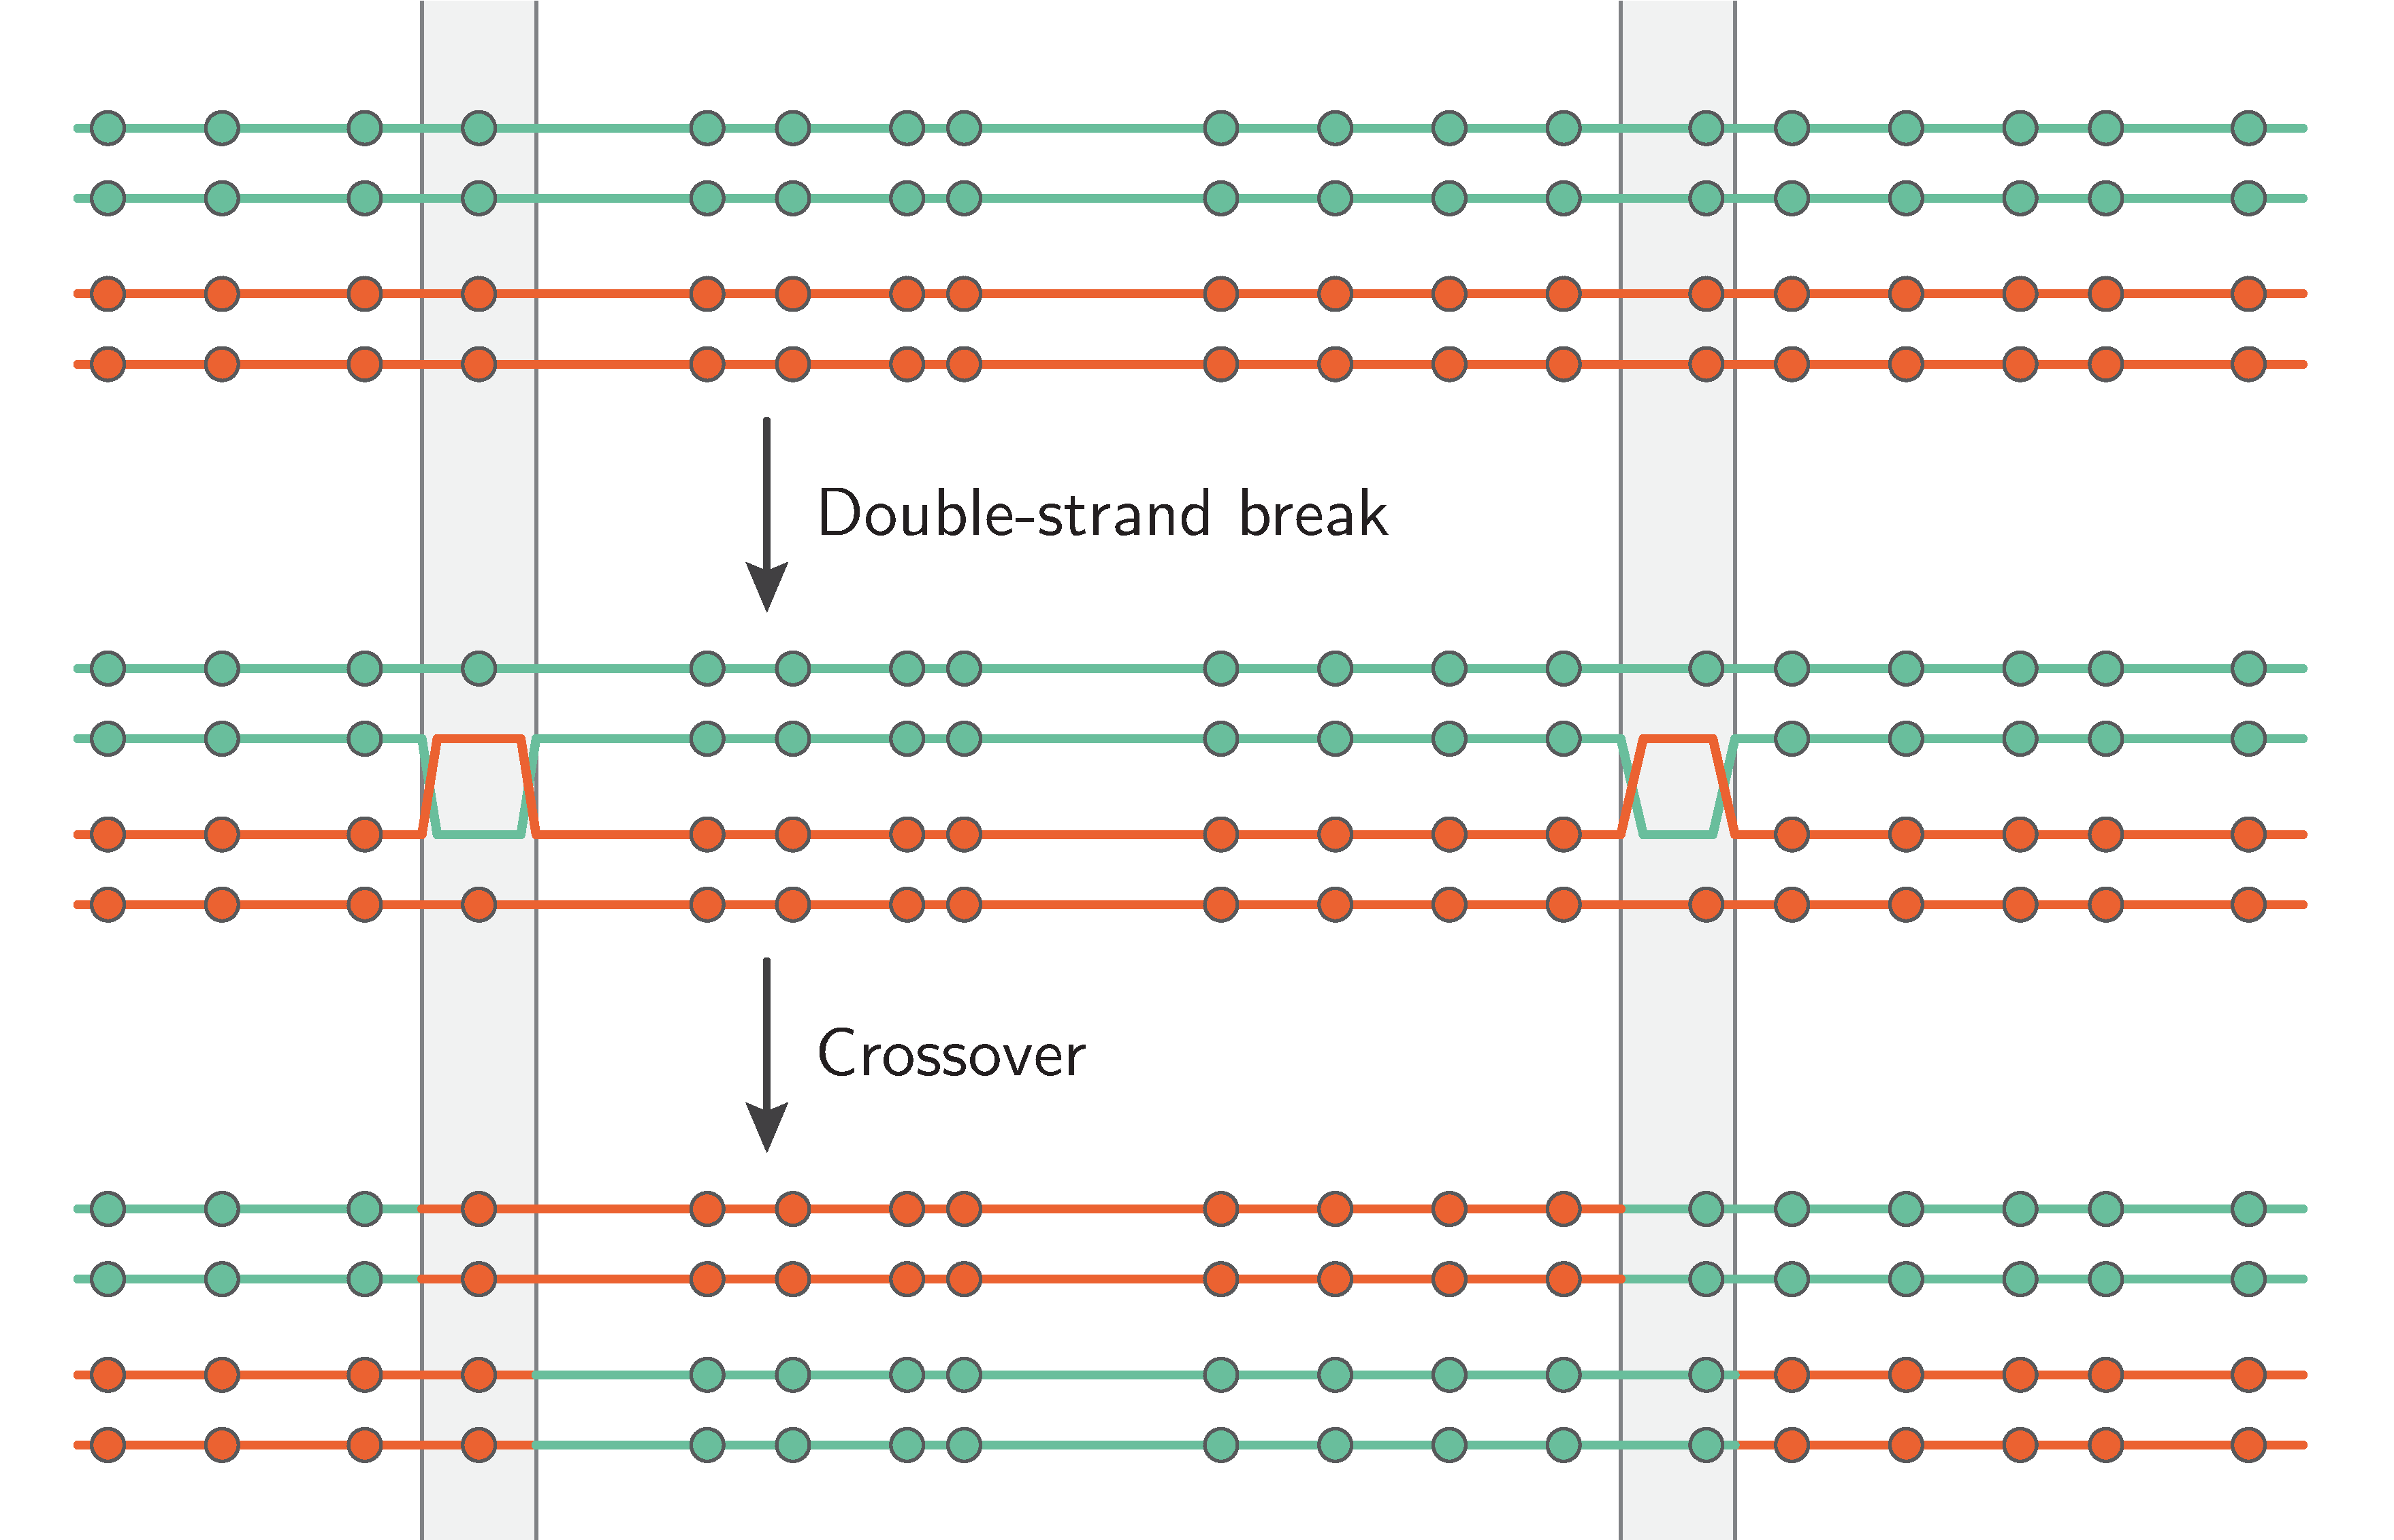
\includegraphics[width=0.8\textwidth]{Images/recombination.pdf}\\
		\caption{ \textbf{ The kingdom of recombinations.} 
}
\end{figure*}

\begin{figure*}[!ht]
	  \centering
       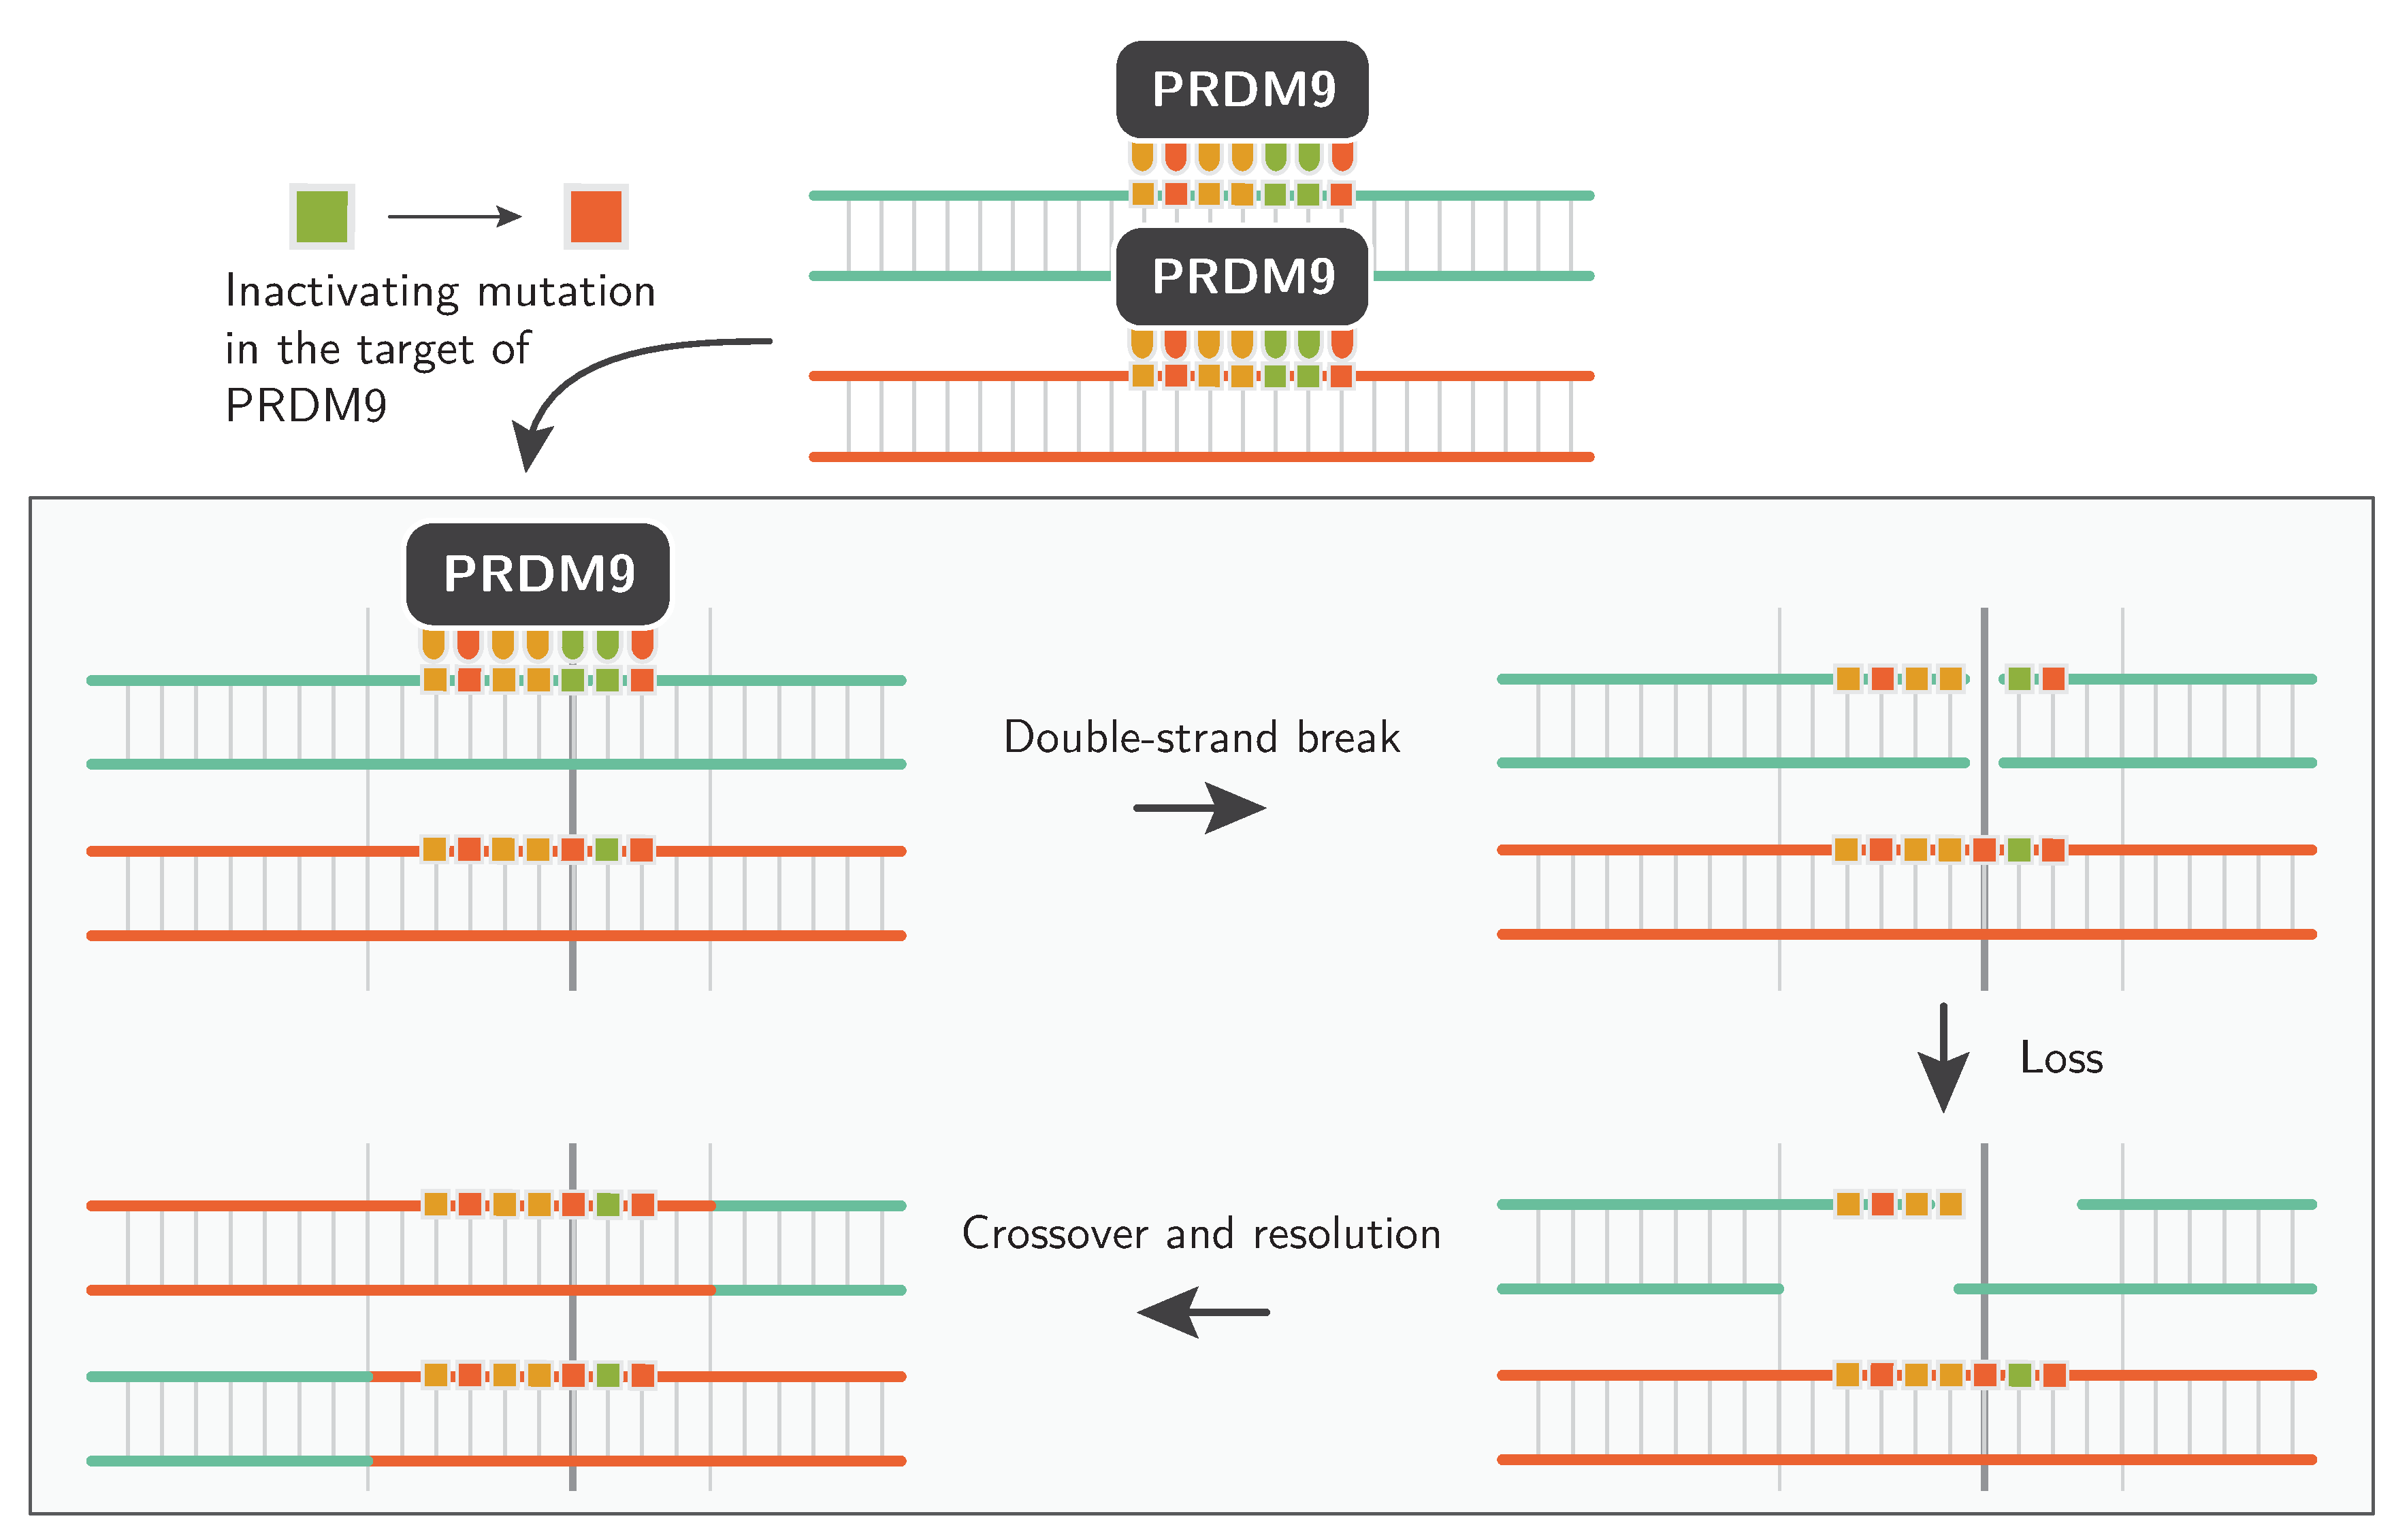
\includegraphics[width=0.8\textwidth]{Images/dBGC.pdf}\\
		\caption{ \textbf{ Biased Gene Conversion.} 
}
\end{figure*}

\begin{figure*}[!ht]
	  \centering
       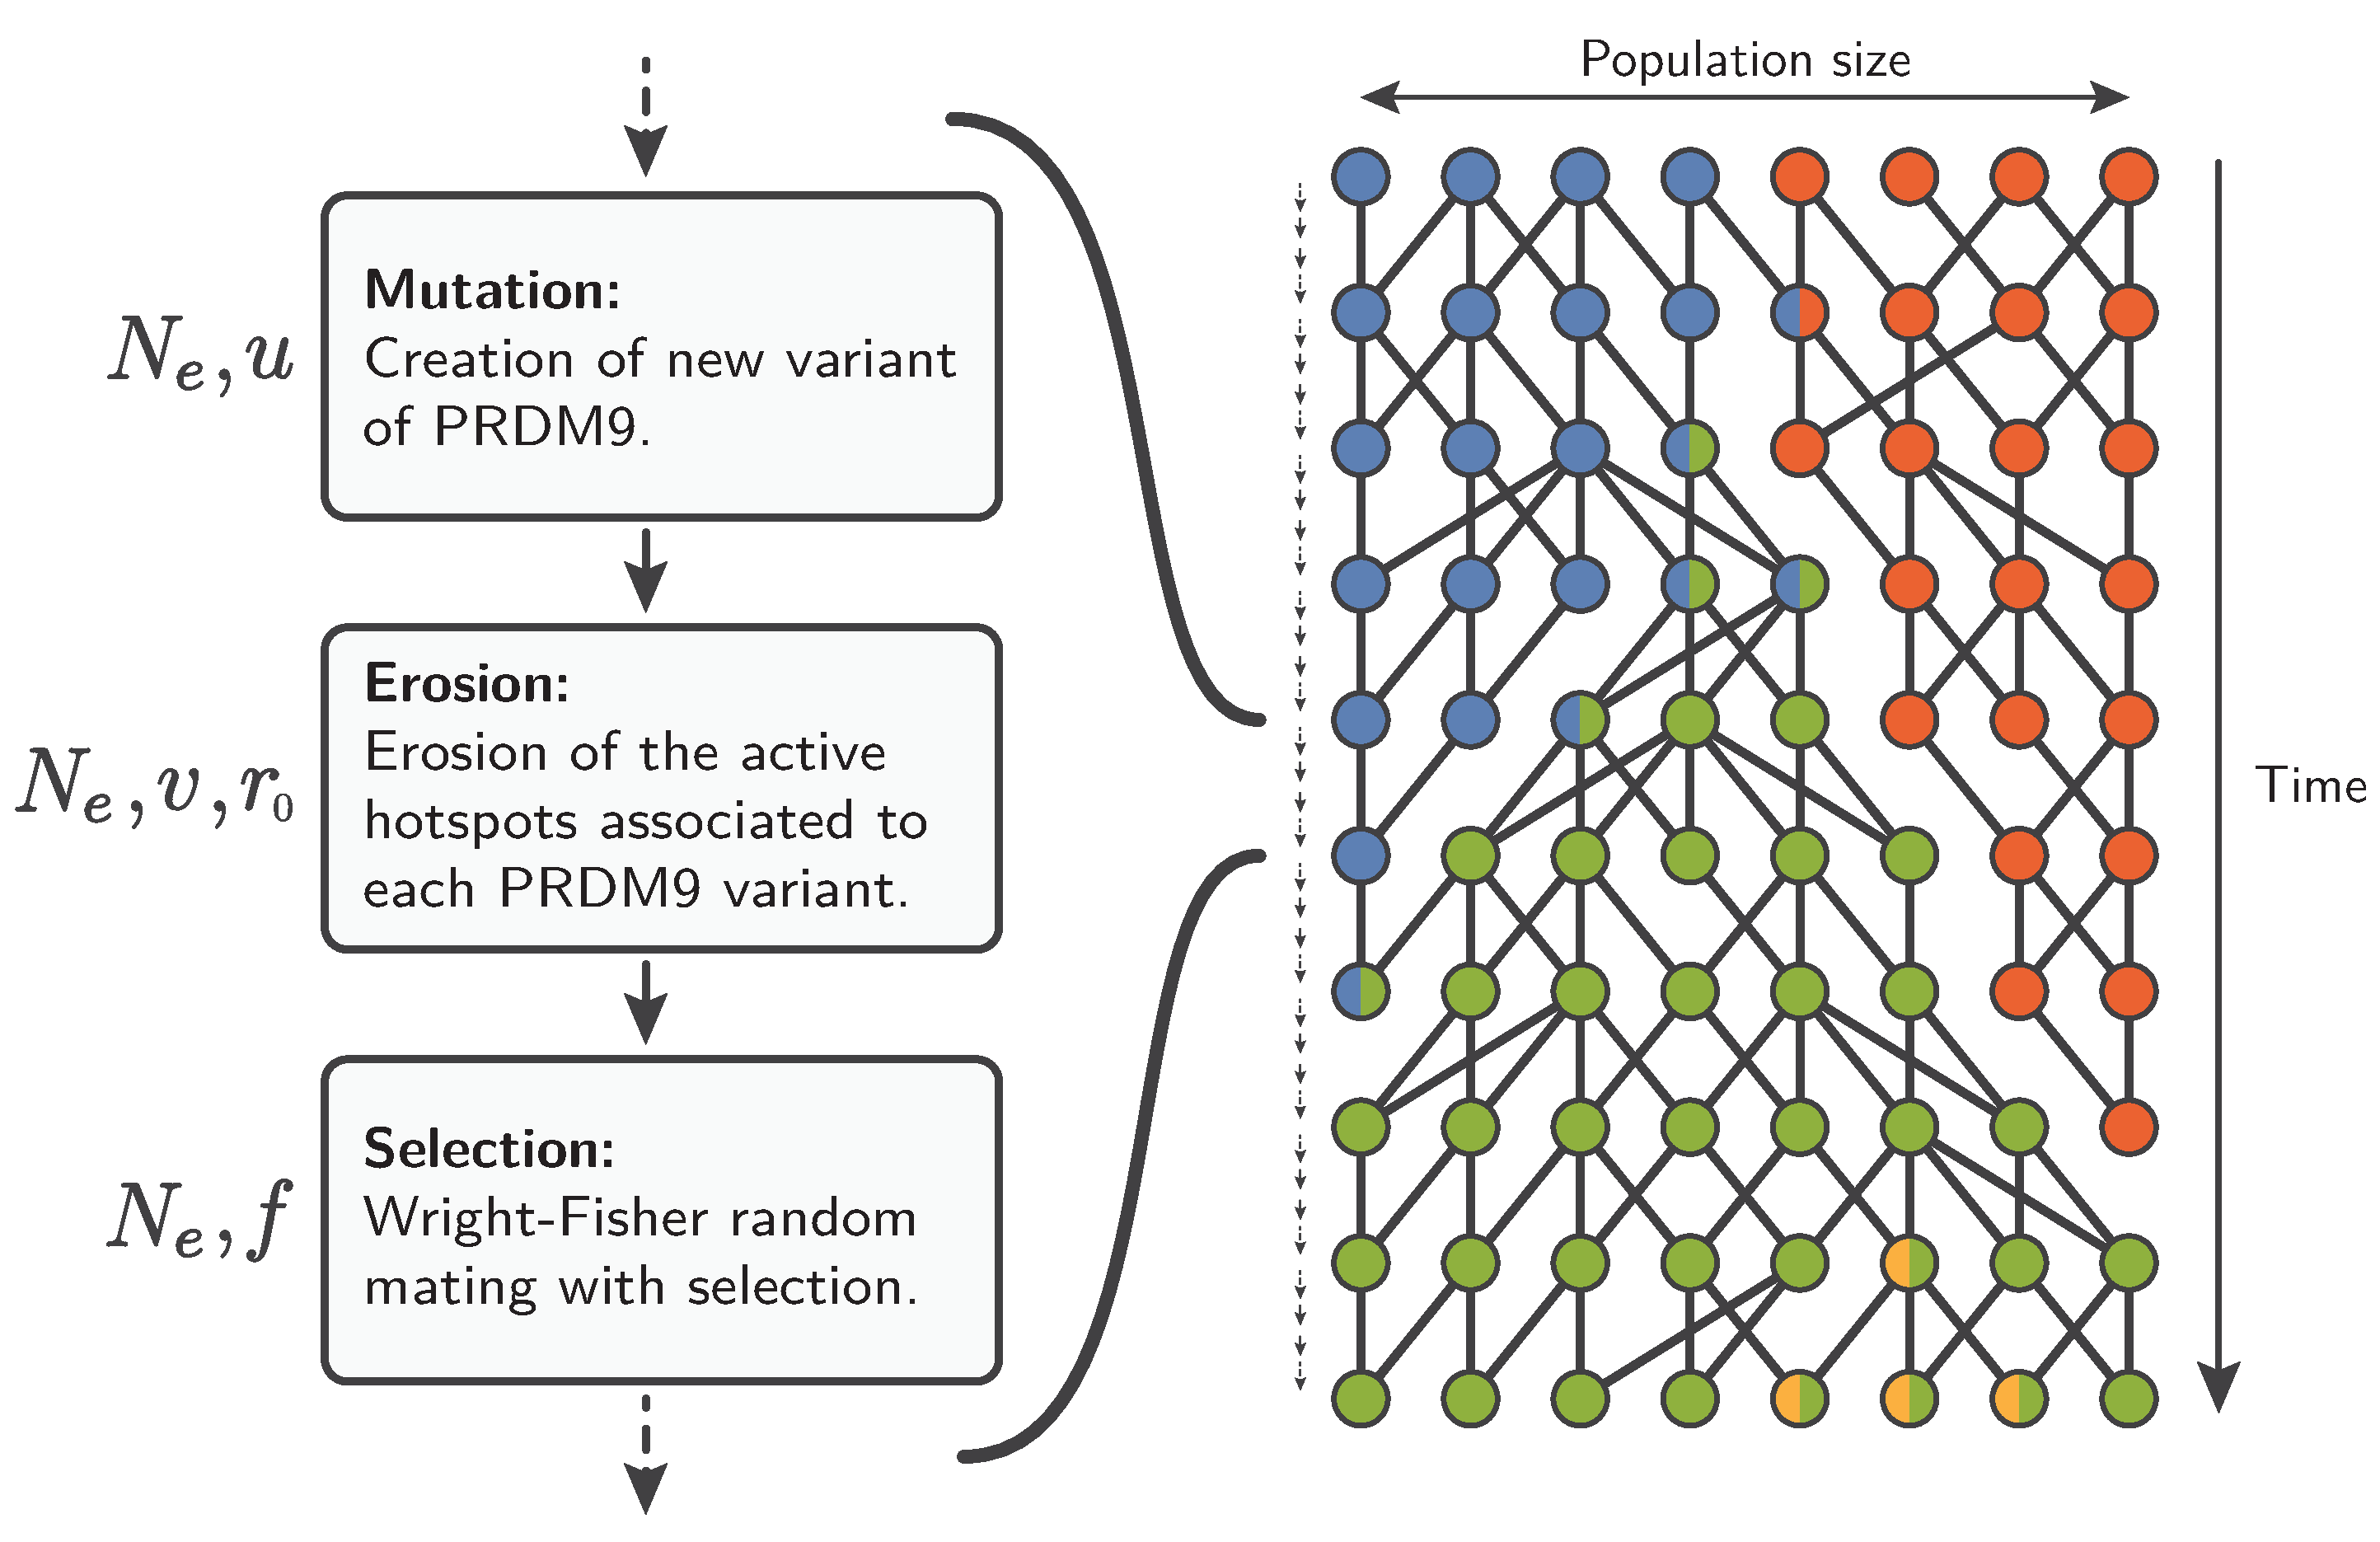
\includegraphics[width=0.8\textwidth]{Images/wright-fisher.pdf}\\
		\caption{ \textbf{ The Wright-Fisher simulator.} 
}
\end{figure*}

\begin{figure*}[!ht]
	  \centering
       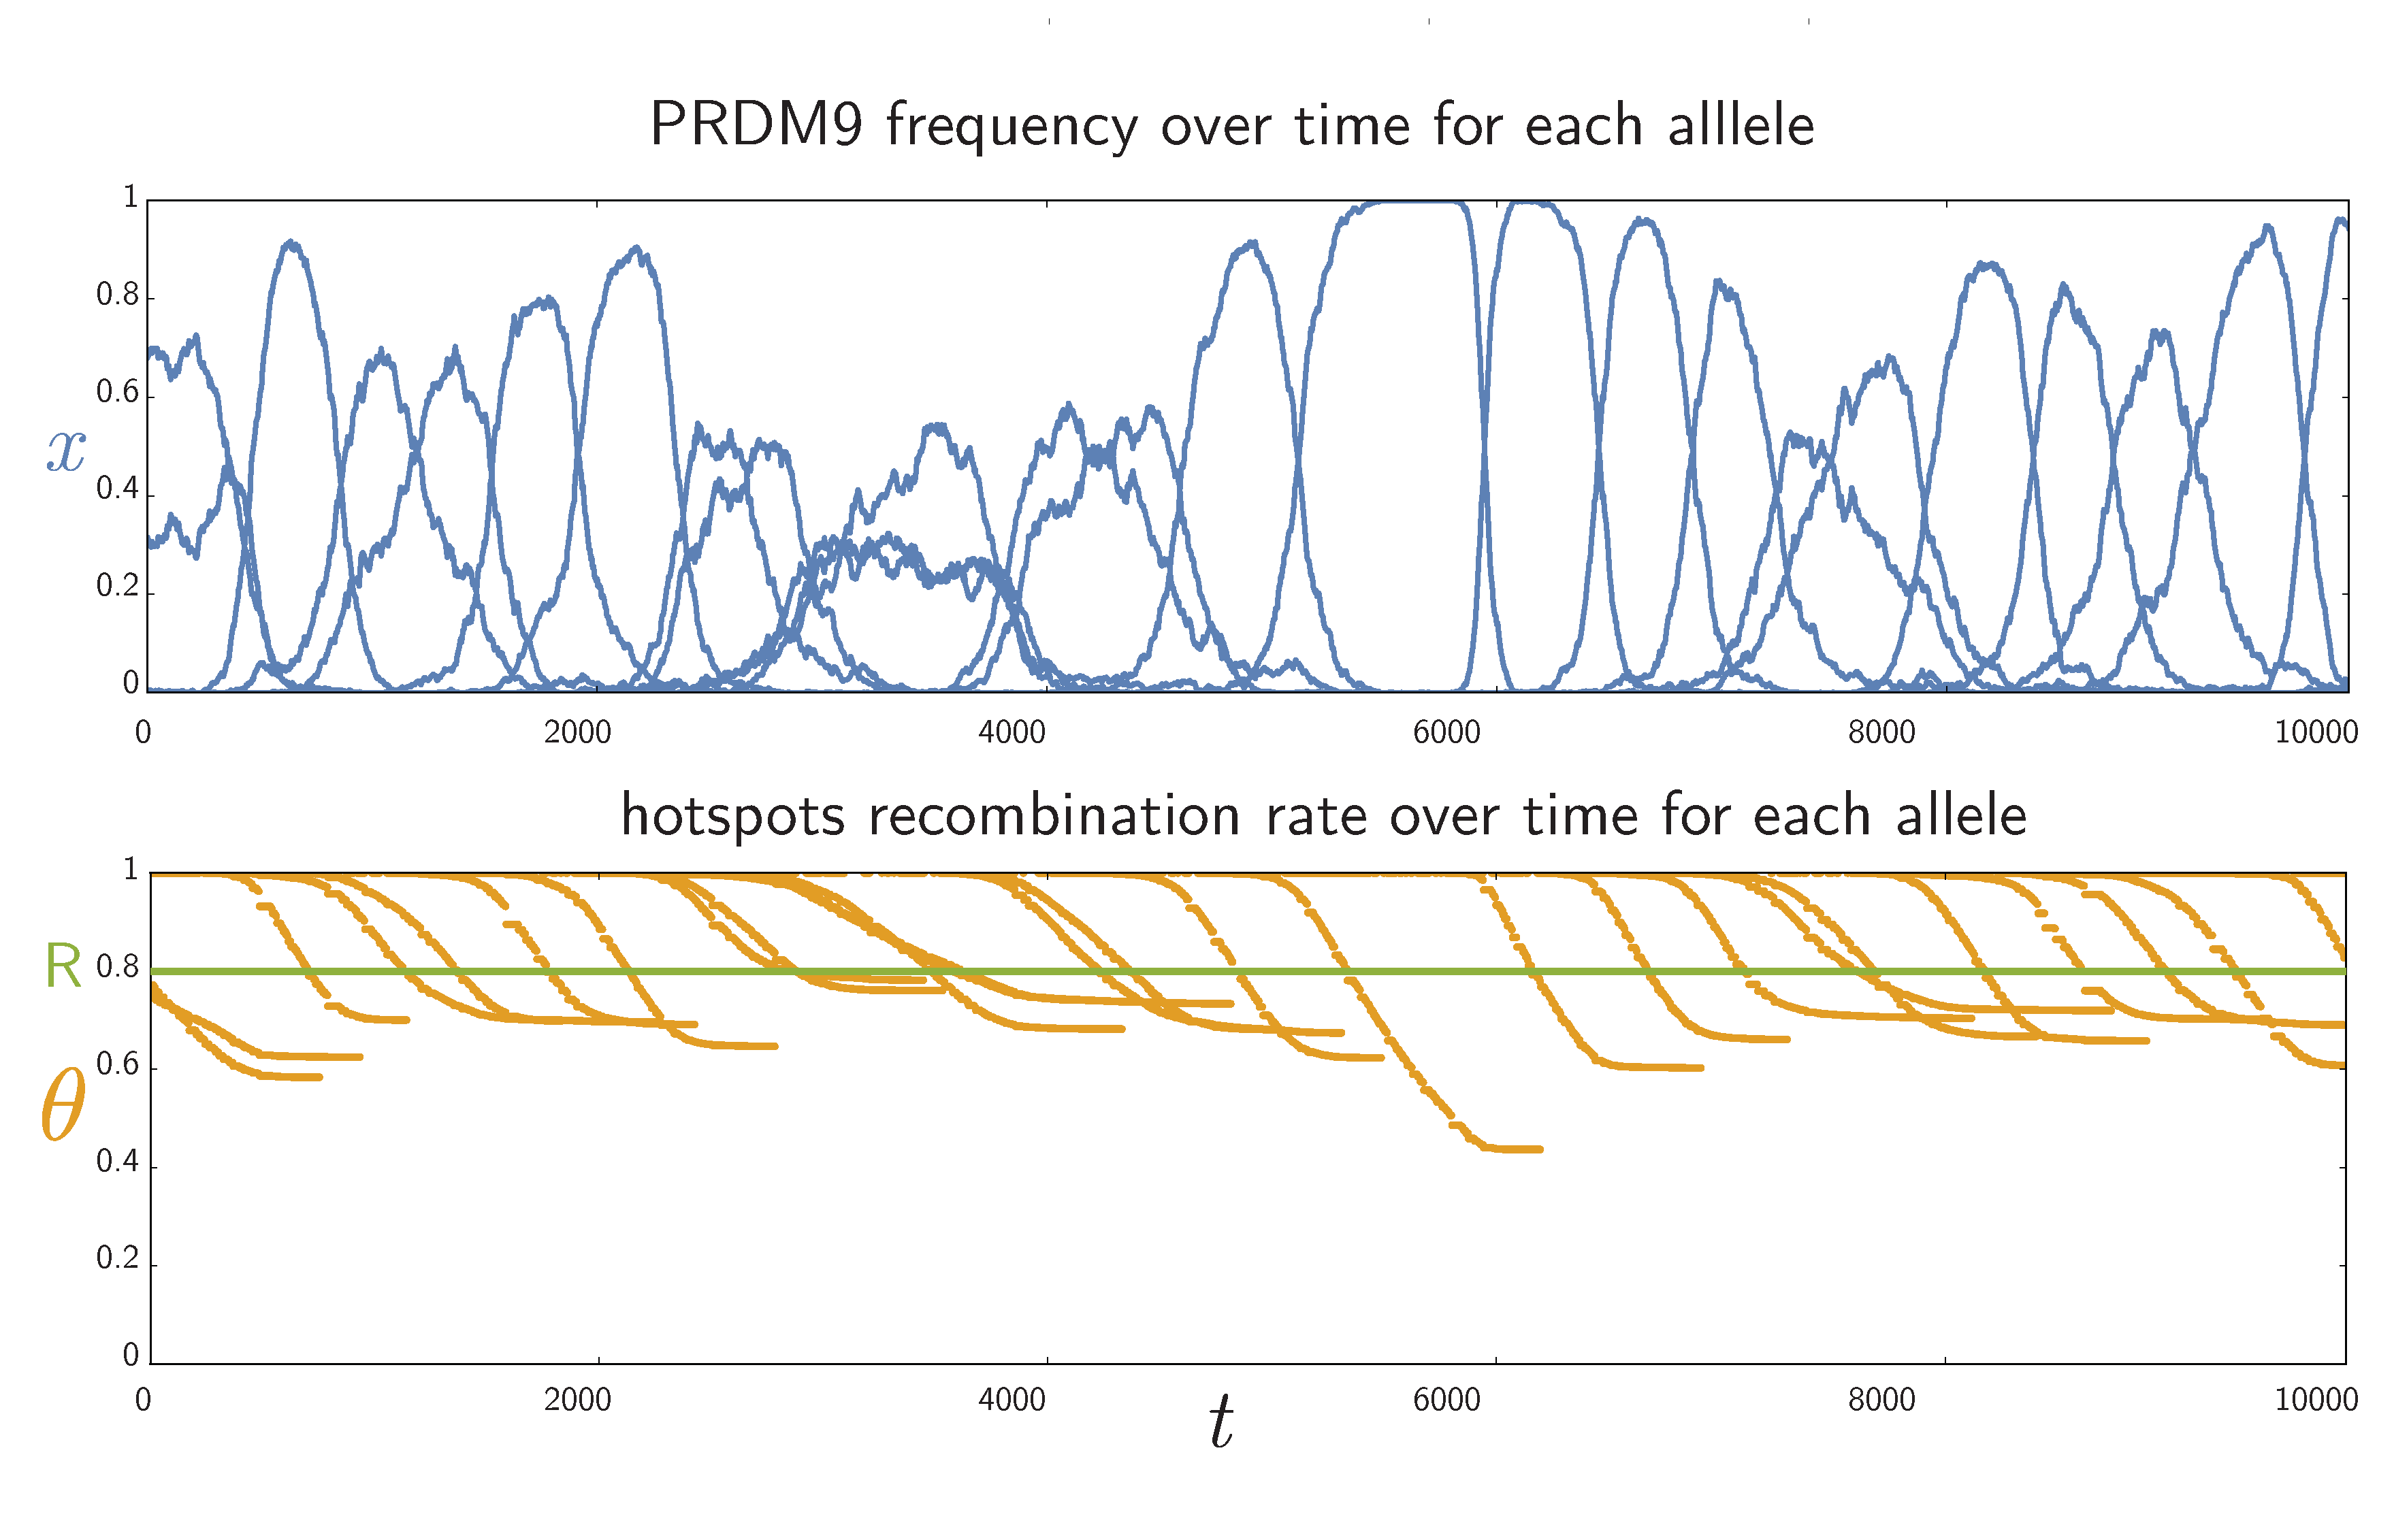
\includegraphics[width=0.8\textwidth]{Images/simulated-trajectory.pdf}\\
		\caption{ \textbf{ Typical simulation trajectory.} 
}
\end{figure*}

\begin{figure*}[!ht]
	  \centering
       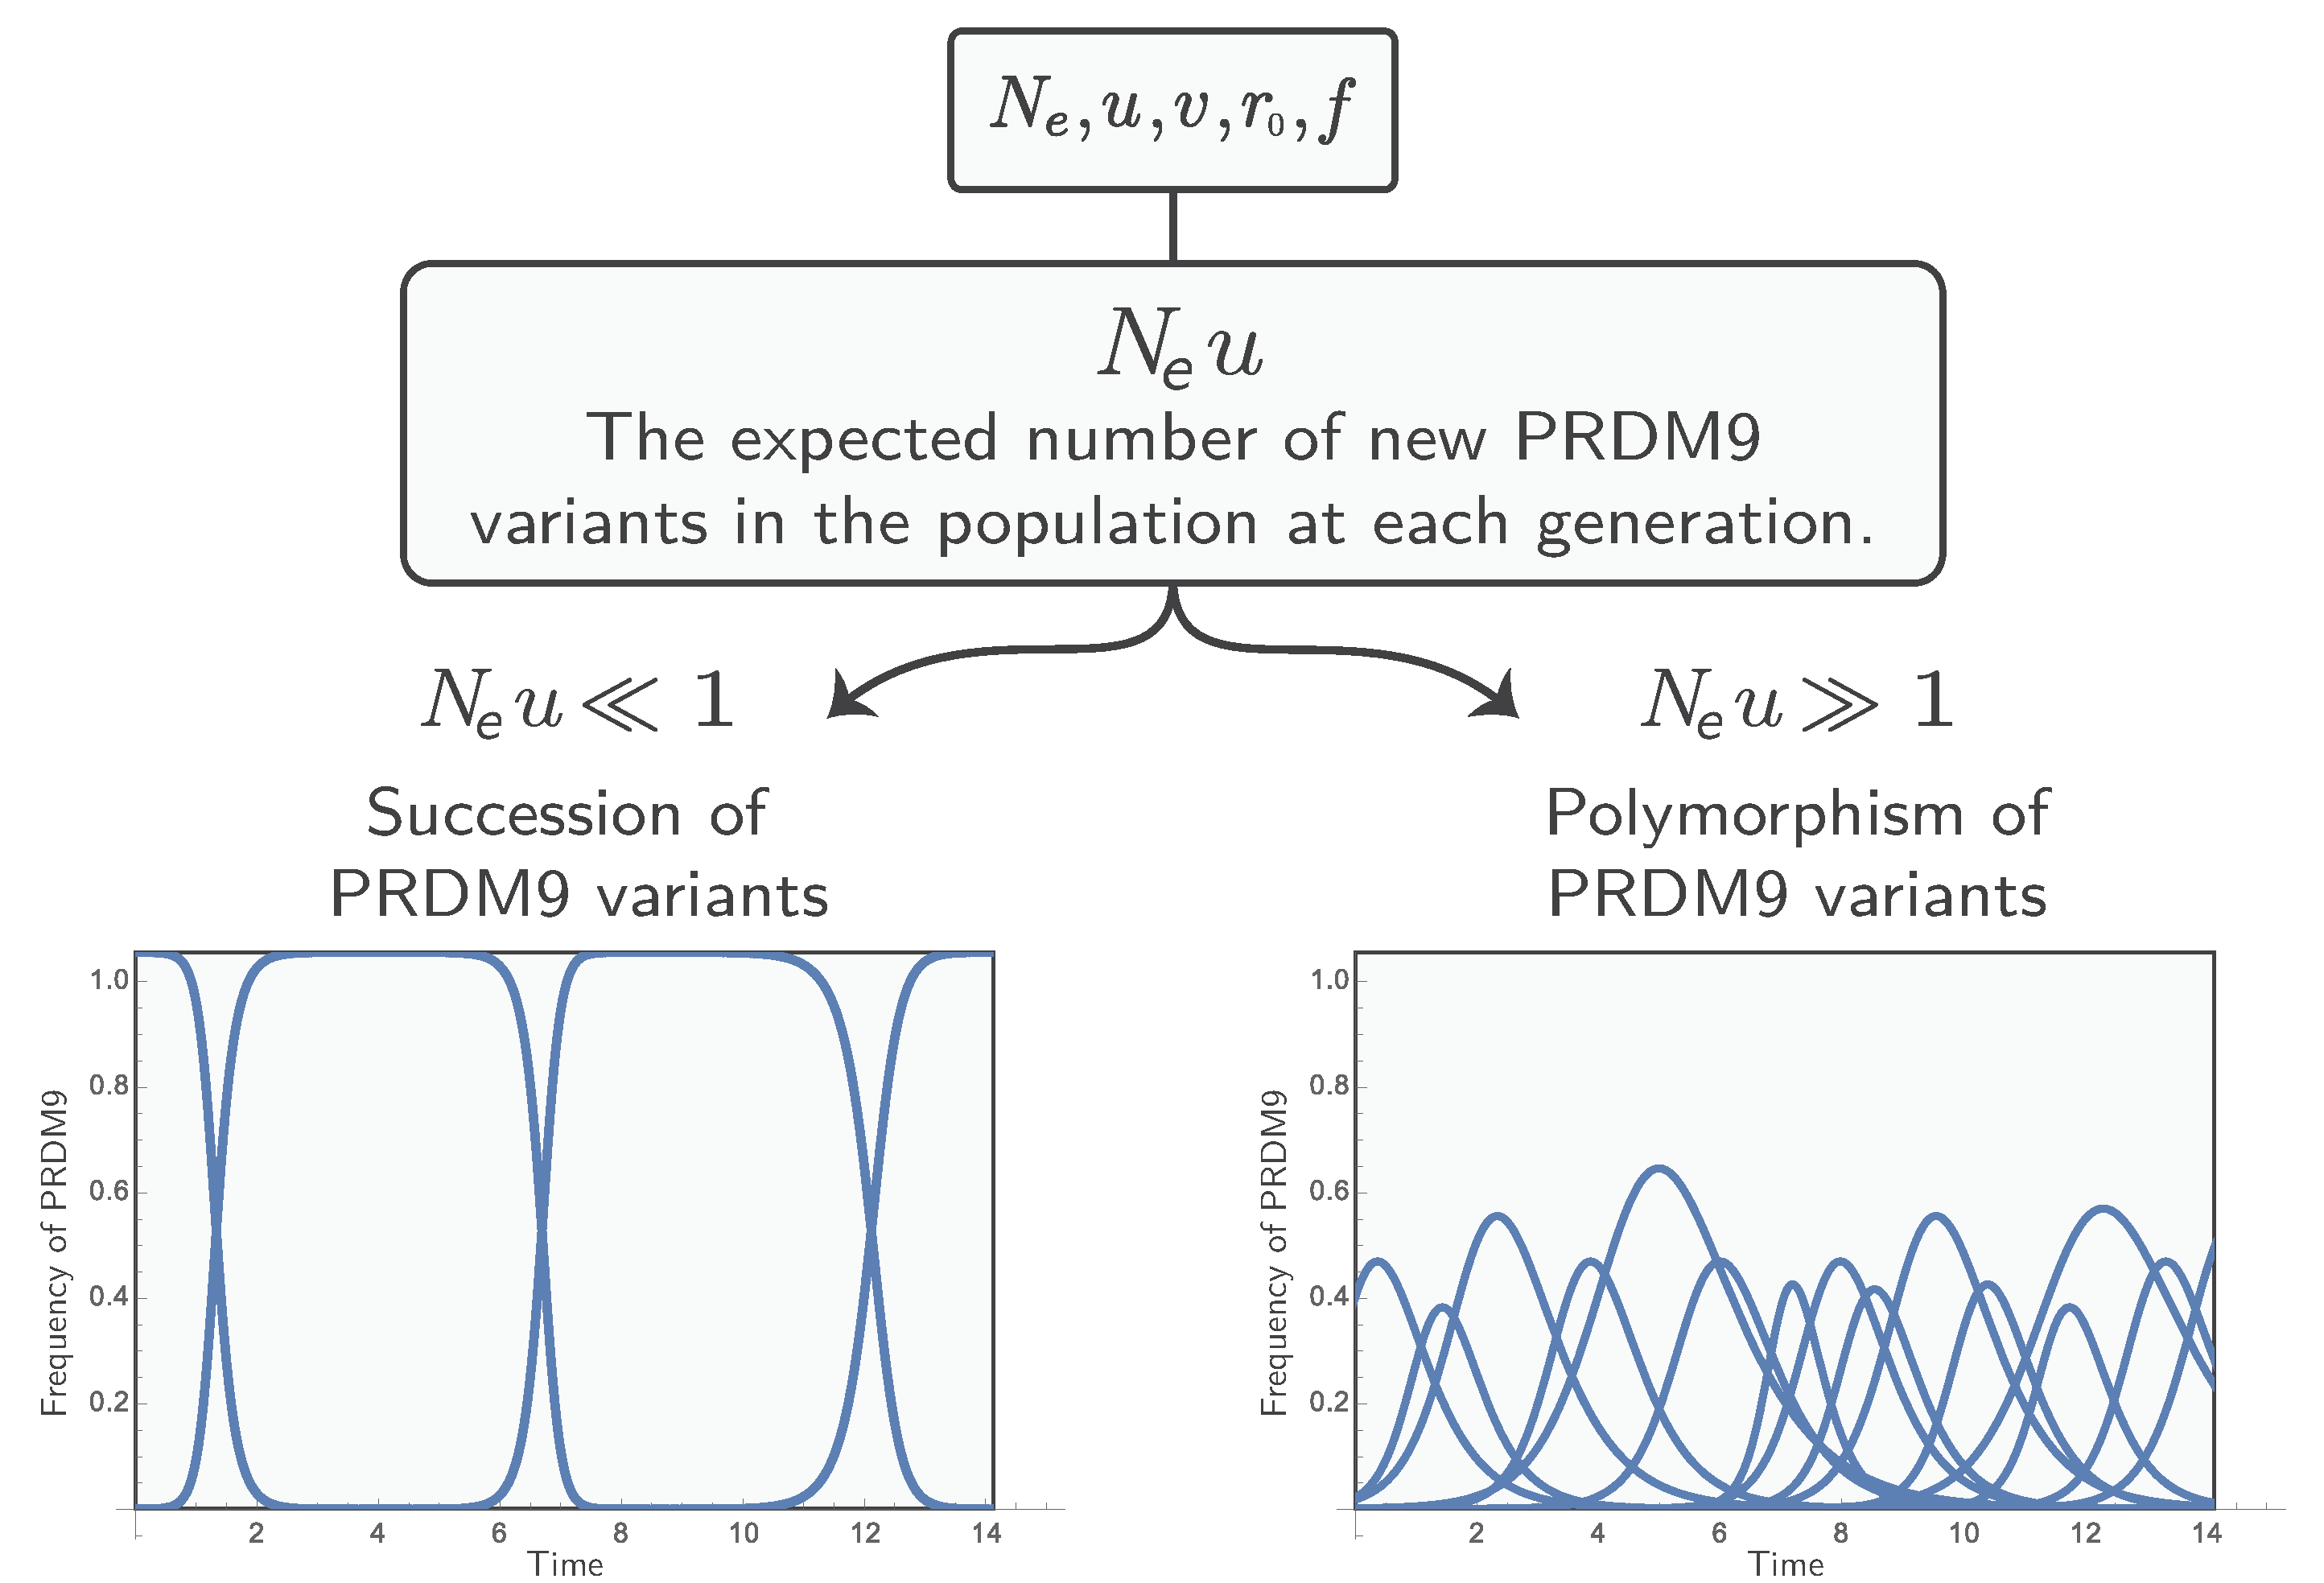
\includegraphics[width=0.8\textwidth]{Images/polymorphism.pdf}\\
		\caption{ \textbf{ Polymorphism or succession ?} 
}
\end{figure*}

\begin{figure*}[!ht]
	  \centering
       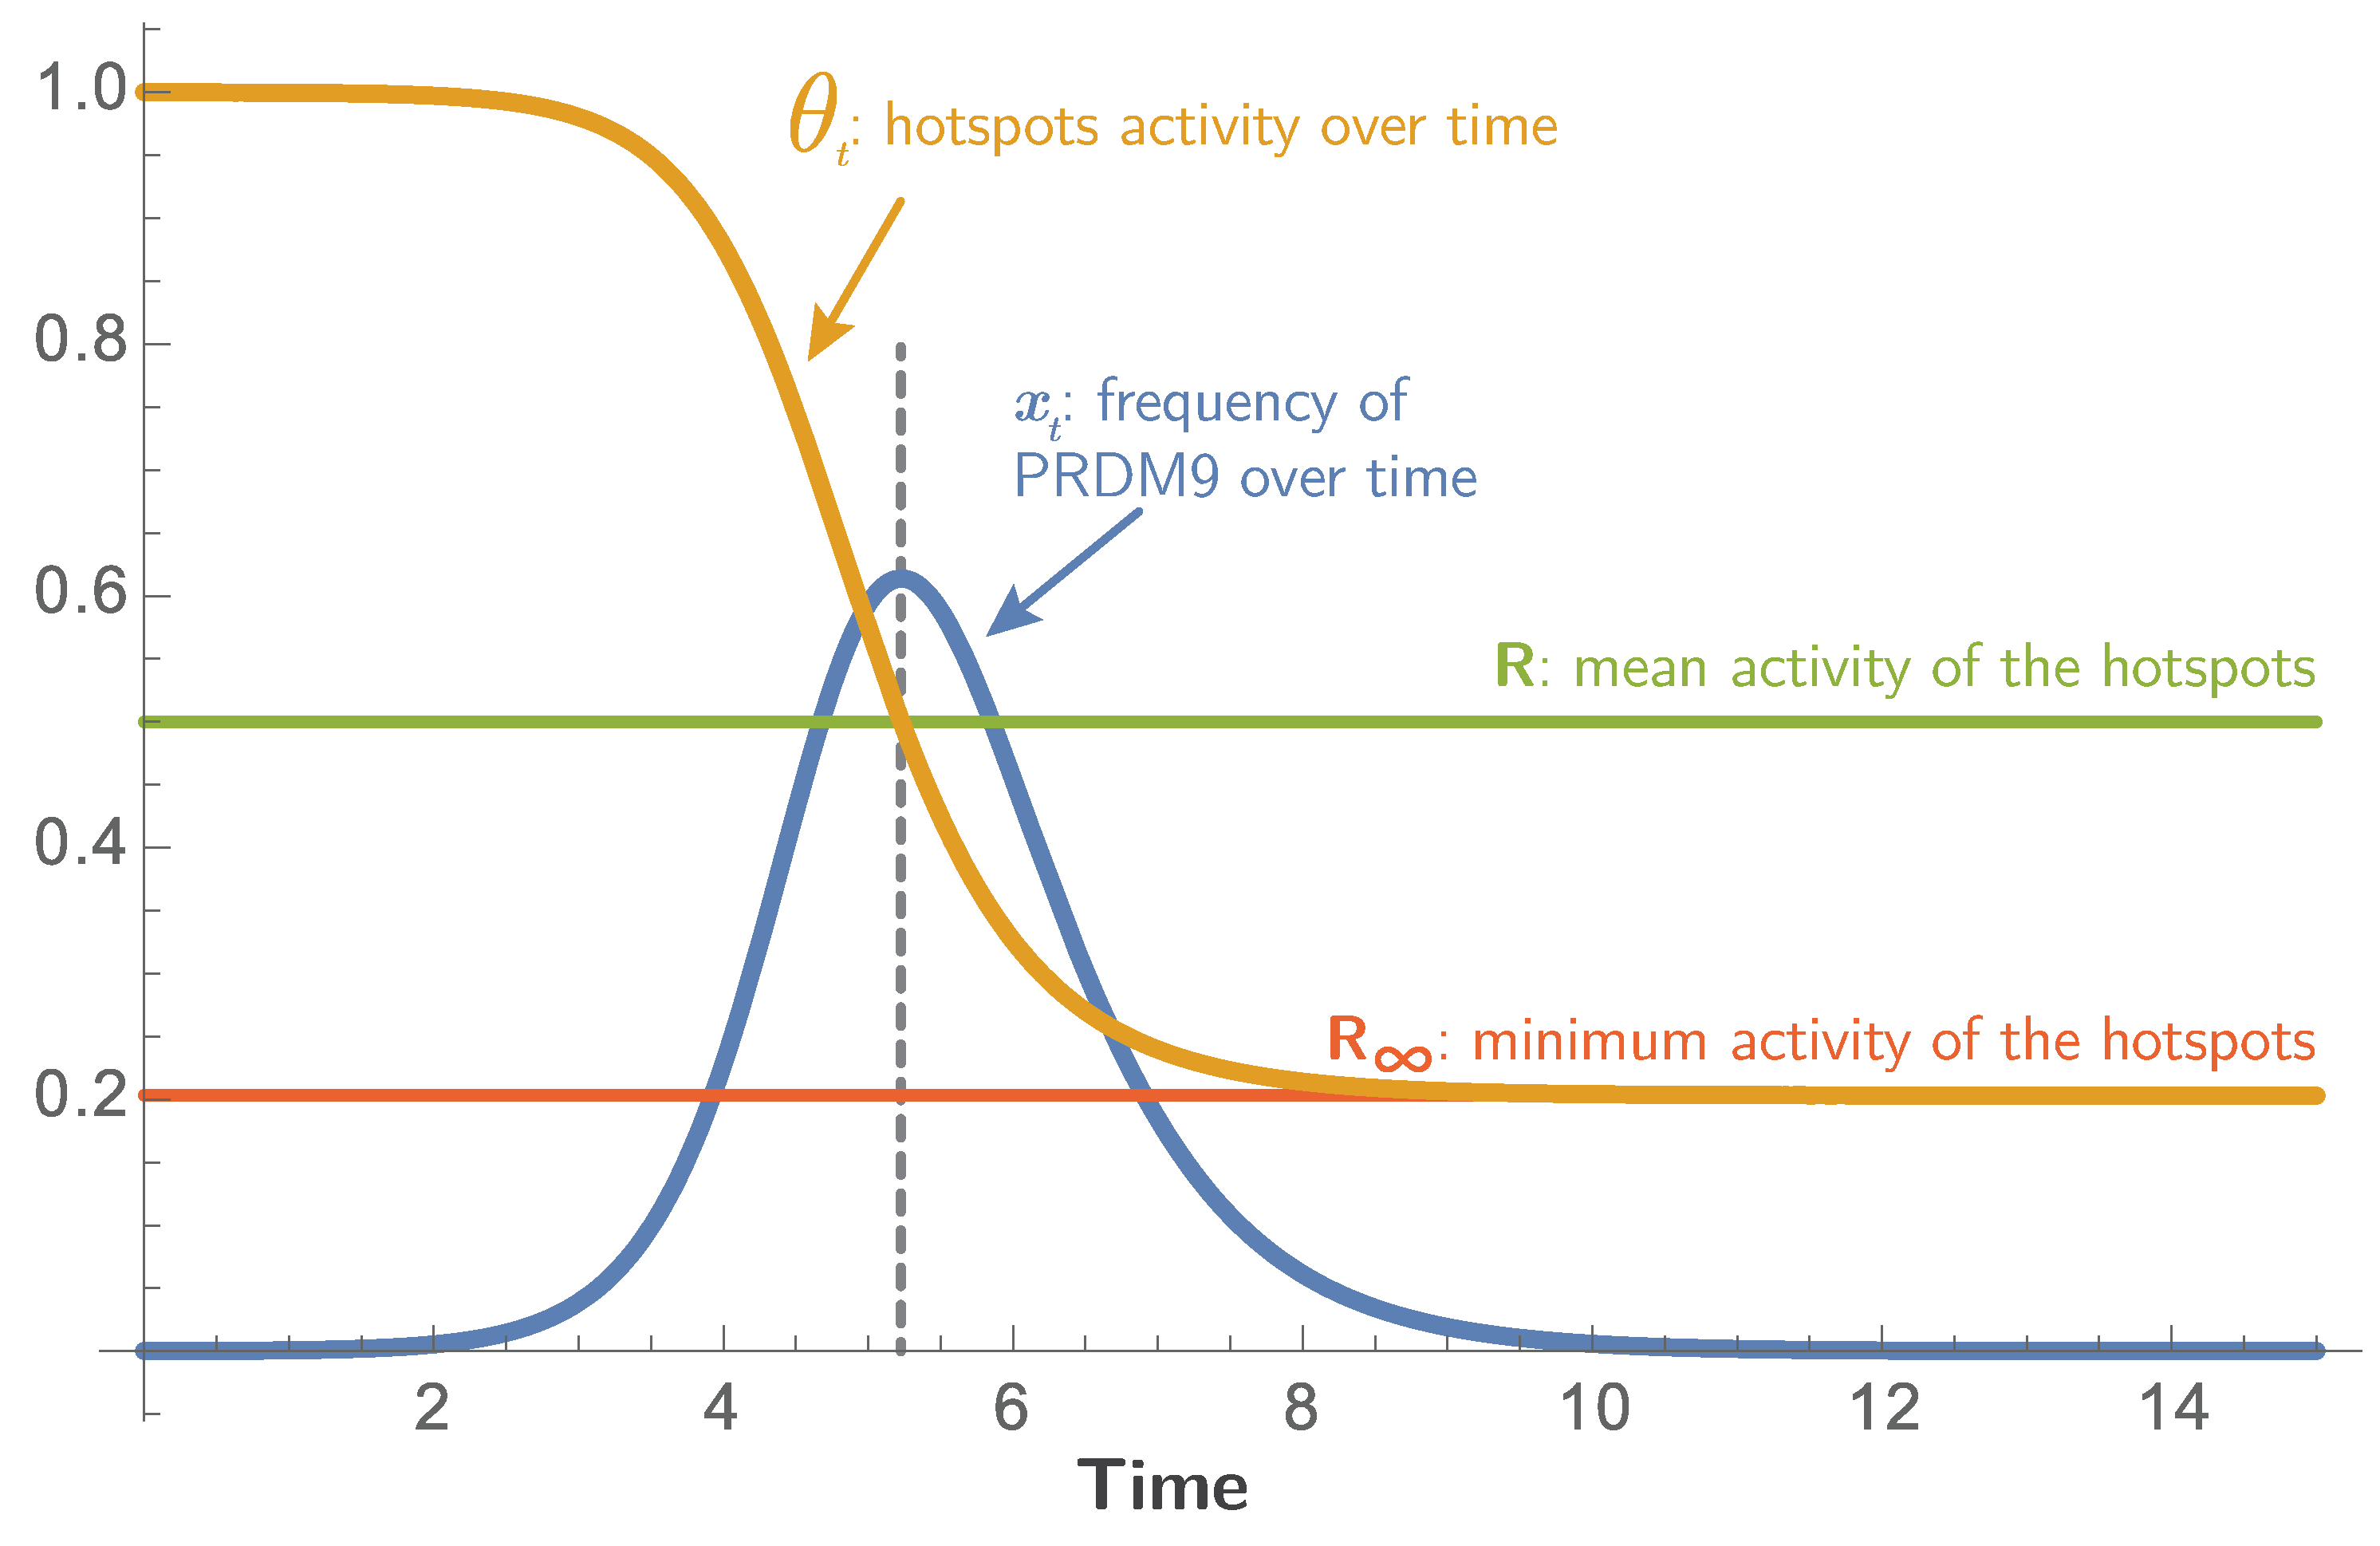
\includegraphics[width=0.8\textwidth]{Images/single-allele.pdf}\\
		\caption{ \textbf{ Trajectory of a single allele} 
}
\end{figure*}

\begin{figure*}[!ht]
	  \centering
       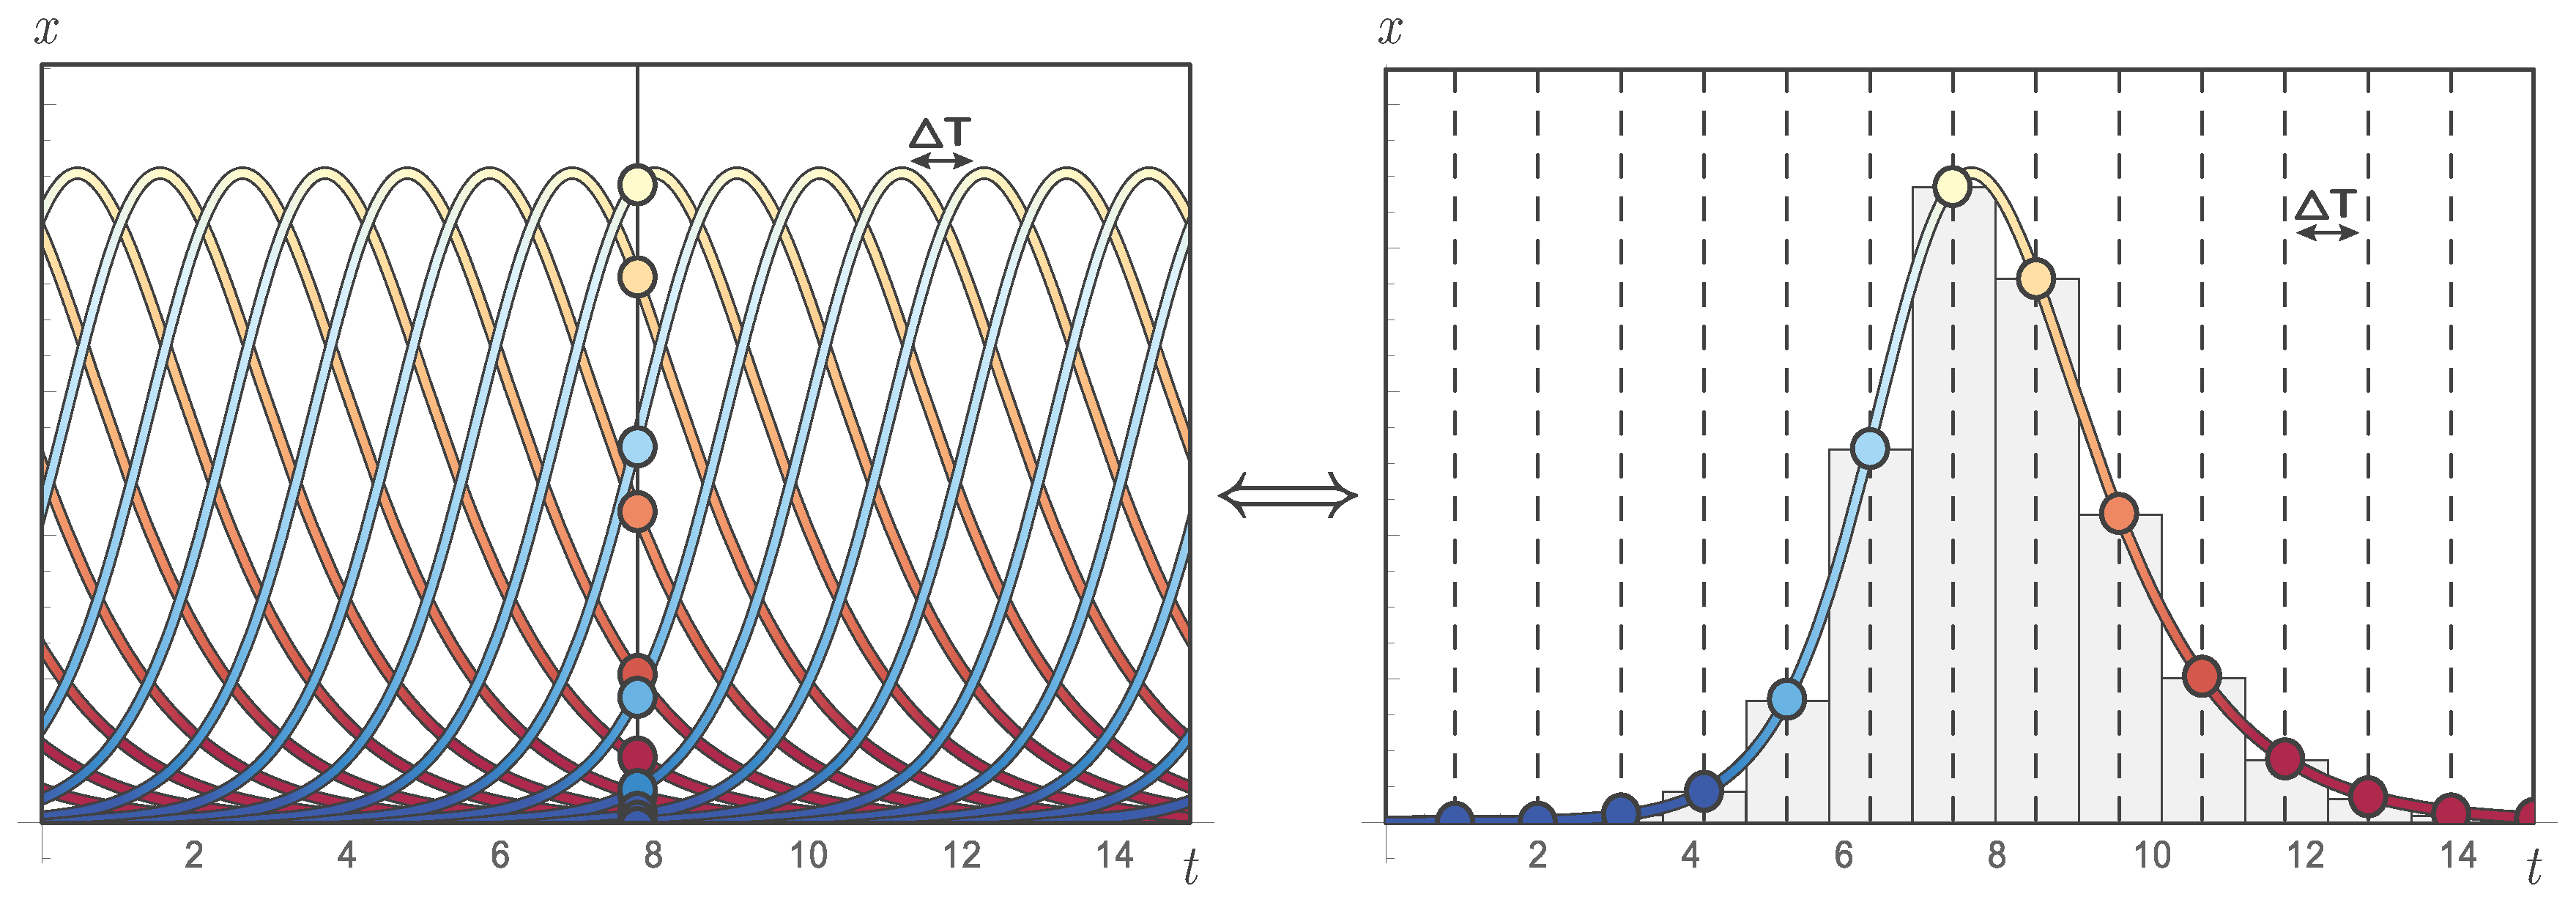
\includegraphics[width=0.8\textwidth]{Images/tilling-argument.pdf}\\
		\caption{ \textbf{ Tilling argument.} 
}
\end{figure*}

\clearpage

\part*{Phase diagram data}
Each simulation starts by a burn-in, and the the data a recorded only when the steady-state is reached. The burn-in phase is finished when all initial alleles in the population are extinct and replaced by new alleles. The number of generations simulated at the steady state is $50$ times the number of generations necessary during burn-in. \\

Each phase diagram is computed by running $16$ independent simulations and changing the value of only one parameter around it's central value. The range around the central value of the parameter is $10^{4}$, meaning the minimum value (the left of the diagram) is $10^2$ times lower than the central value, and maximum value (the right of the diagram) is $10^2$ times greater than the central value.\\


The central value for all phase diagrams are :
\begin{itemize}
\item $\Ne=10^{5}$ : The population size
\item $u=10^{-6}$ : The mutation rate at the PRDM9 locus
\item $v=10^{-6}$ : The mutation rate at the hotspots locus
\item $r_0=10^{-3}$ : The recombination rate of active targets
\item $\alpha=10^{-1}$ : The exponent of the fitness function
\end{itemize}

In solid blue are the summary statistics averaged for each simulation.
The range in light blue is the variance (over the simulation) of the summary statistic for each the simulation.

\clearpage

\section*{Self-consistent mean field approximation}
In solid yellow are the summary statistics estimated from the parameters by self-consistent mean field approximation
\begin{figure*}[!ht]
	  \centering
       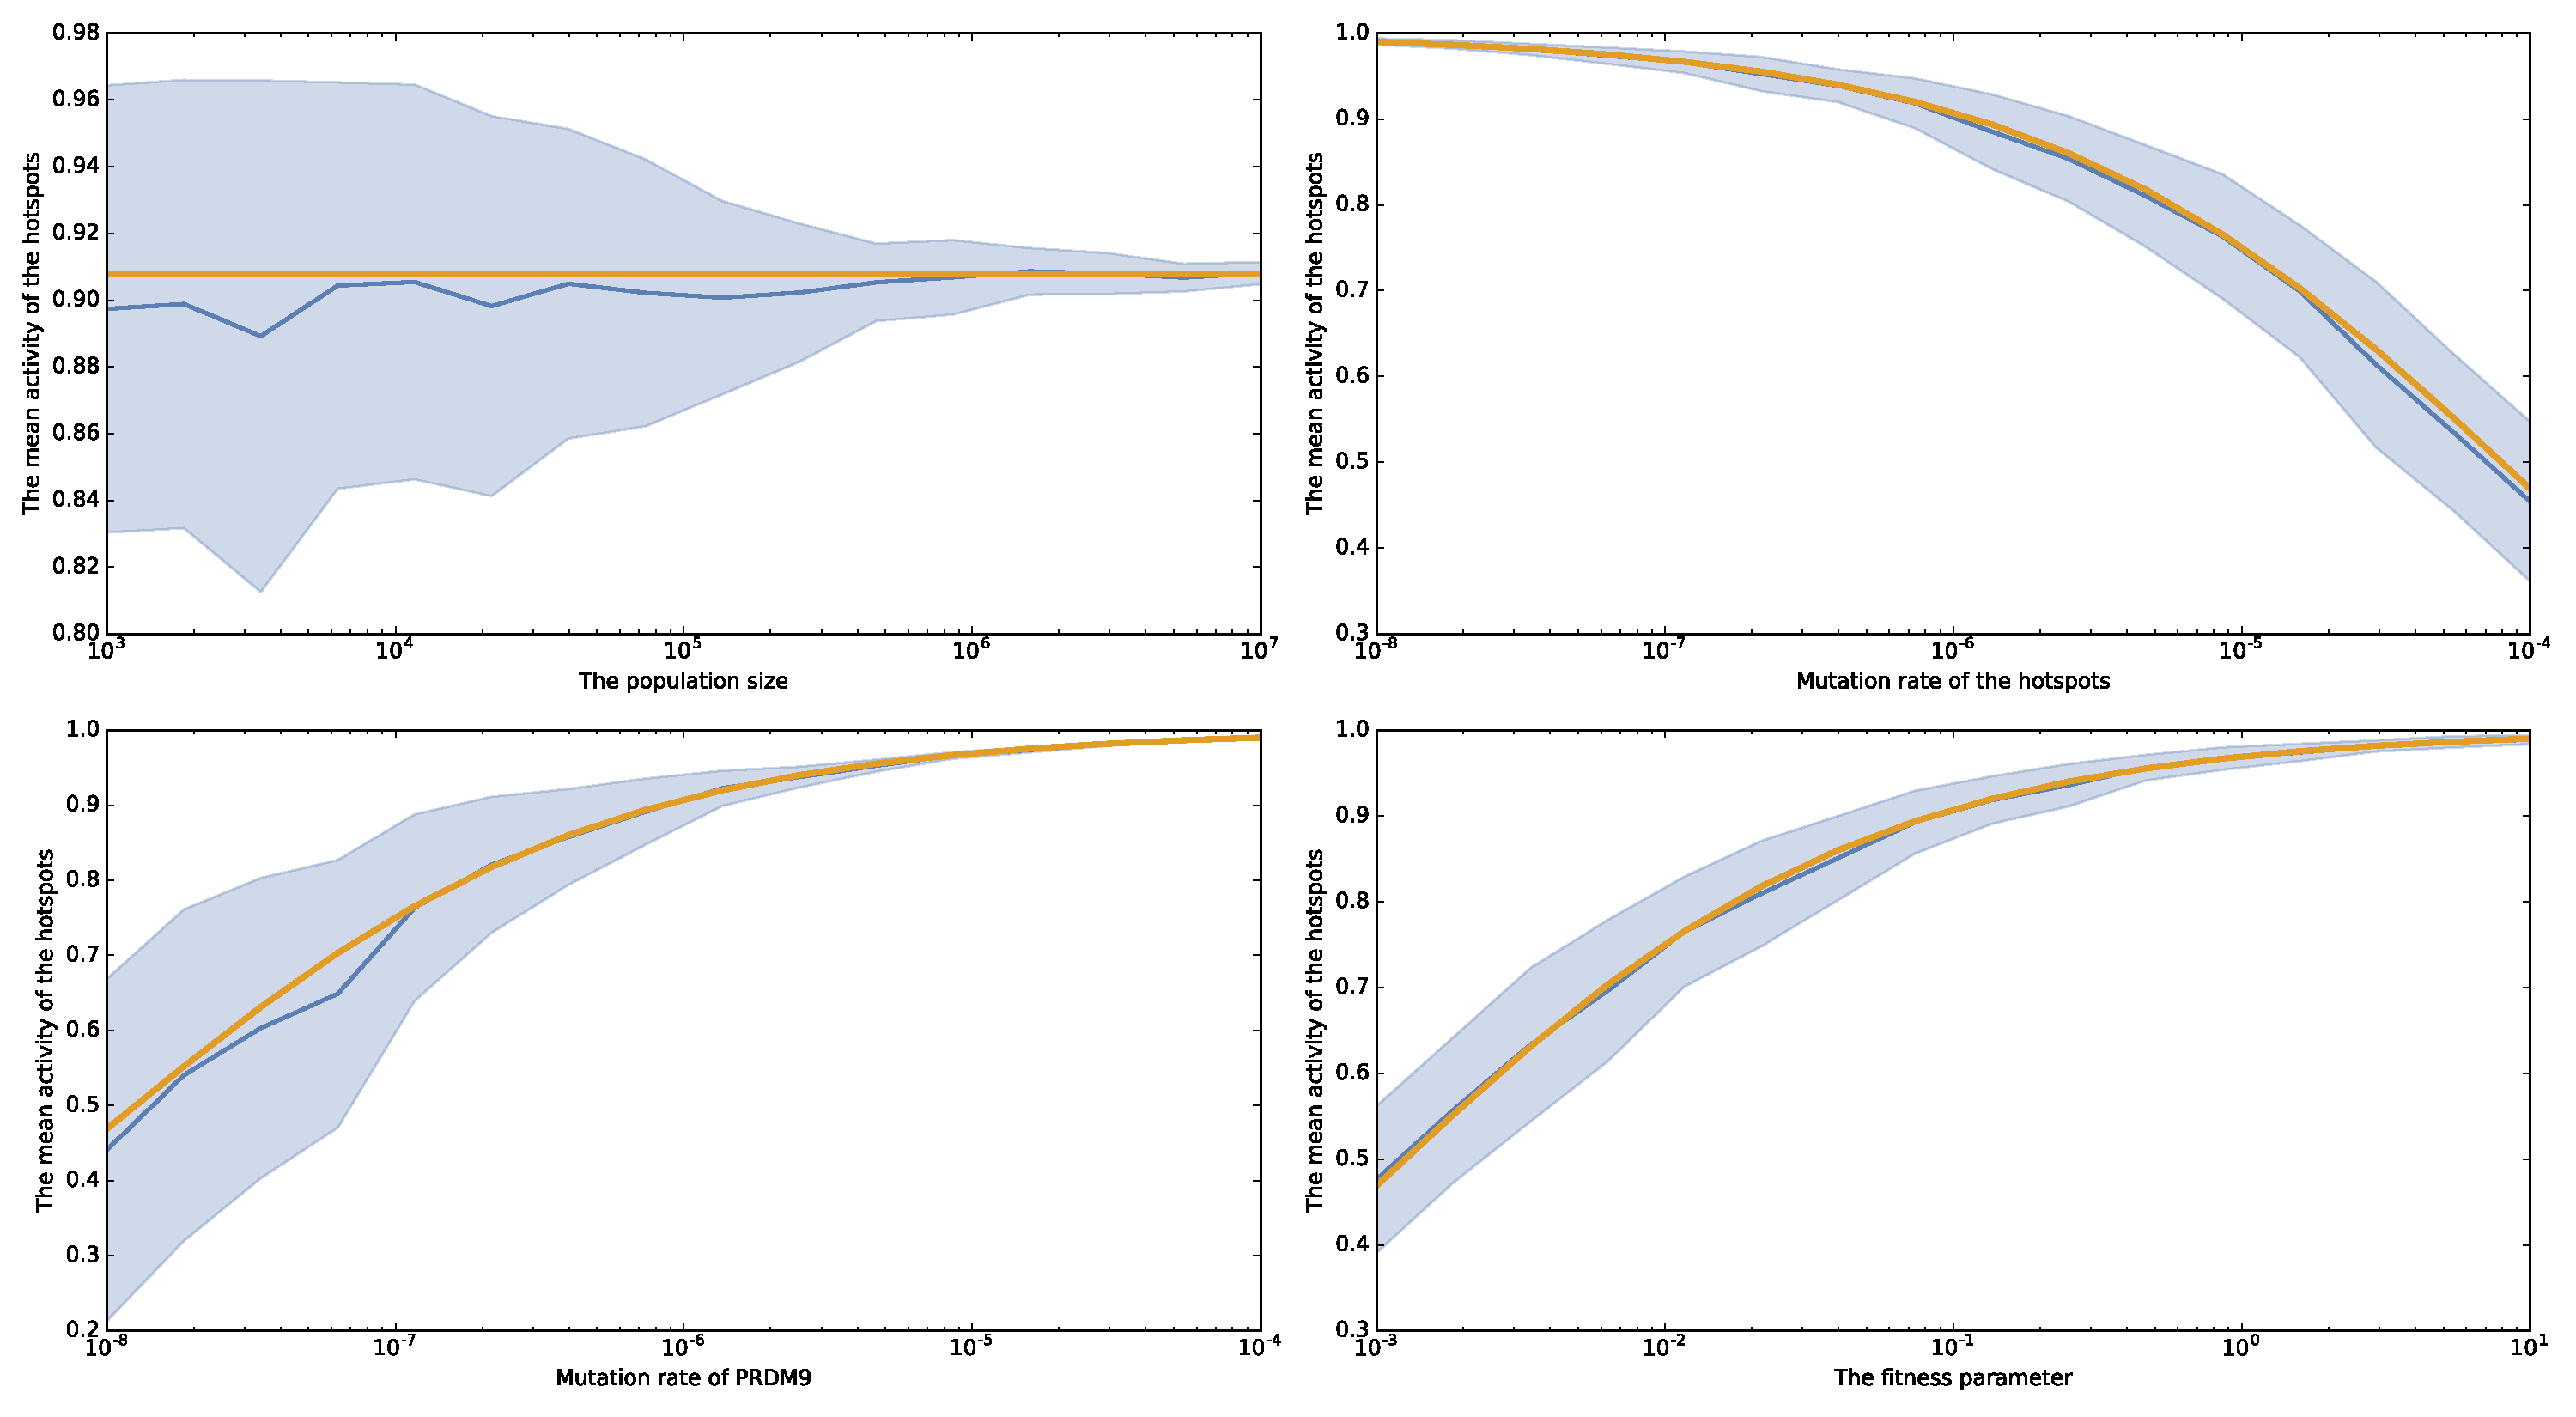
\includegraphics[width=0.8\textwidth]{Images/mean-field-mean-activity.pdf}\\
		\caption{ \textbf{ Mean activity.} 
}
\end{figure*}

\begin{figure*}[!ht]
	  \centering
       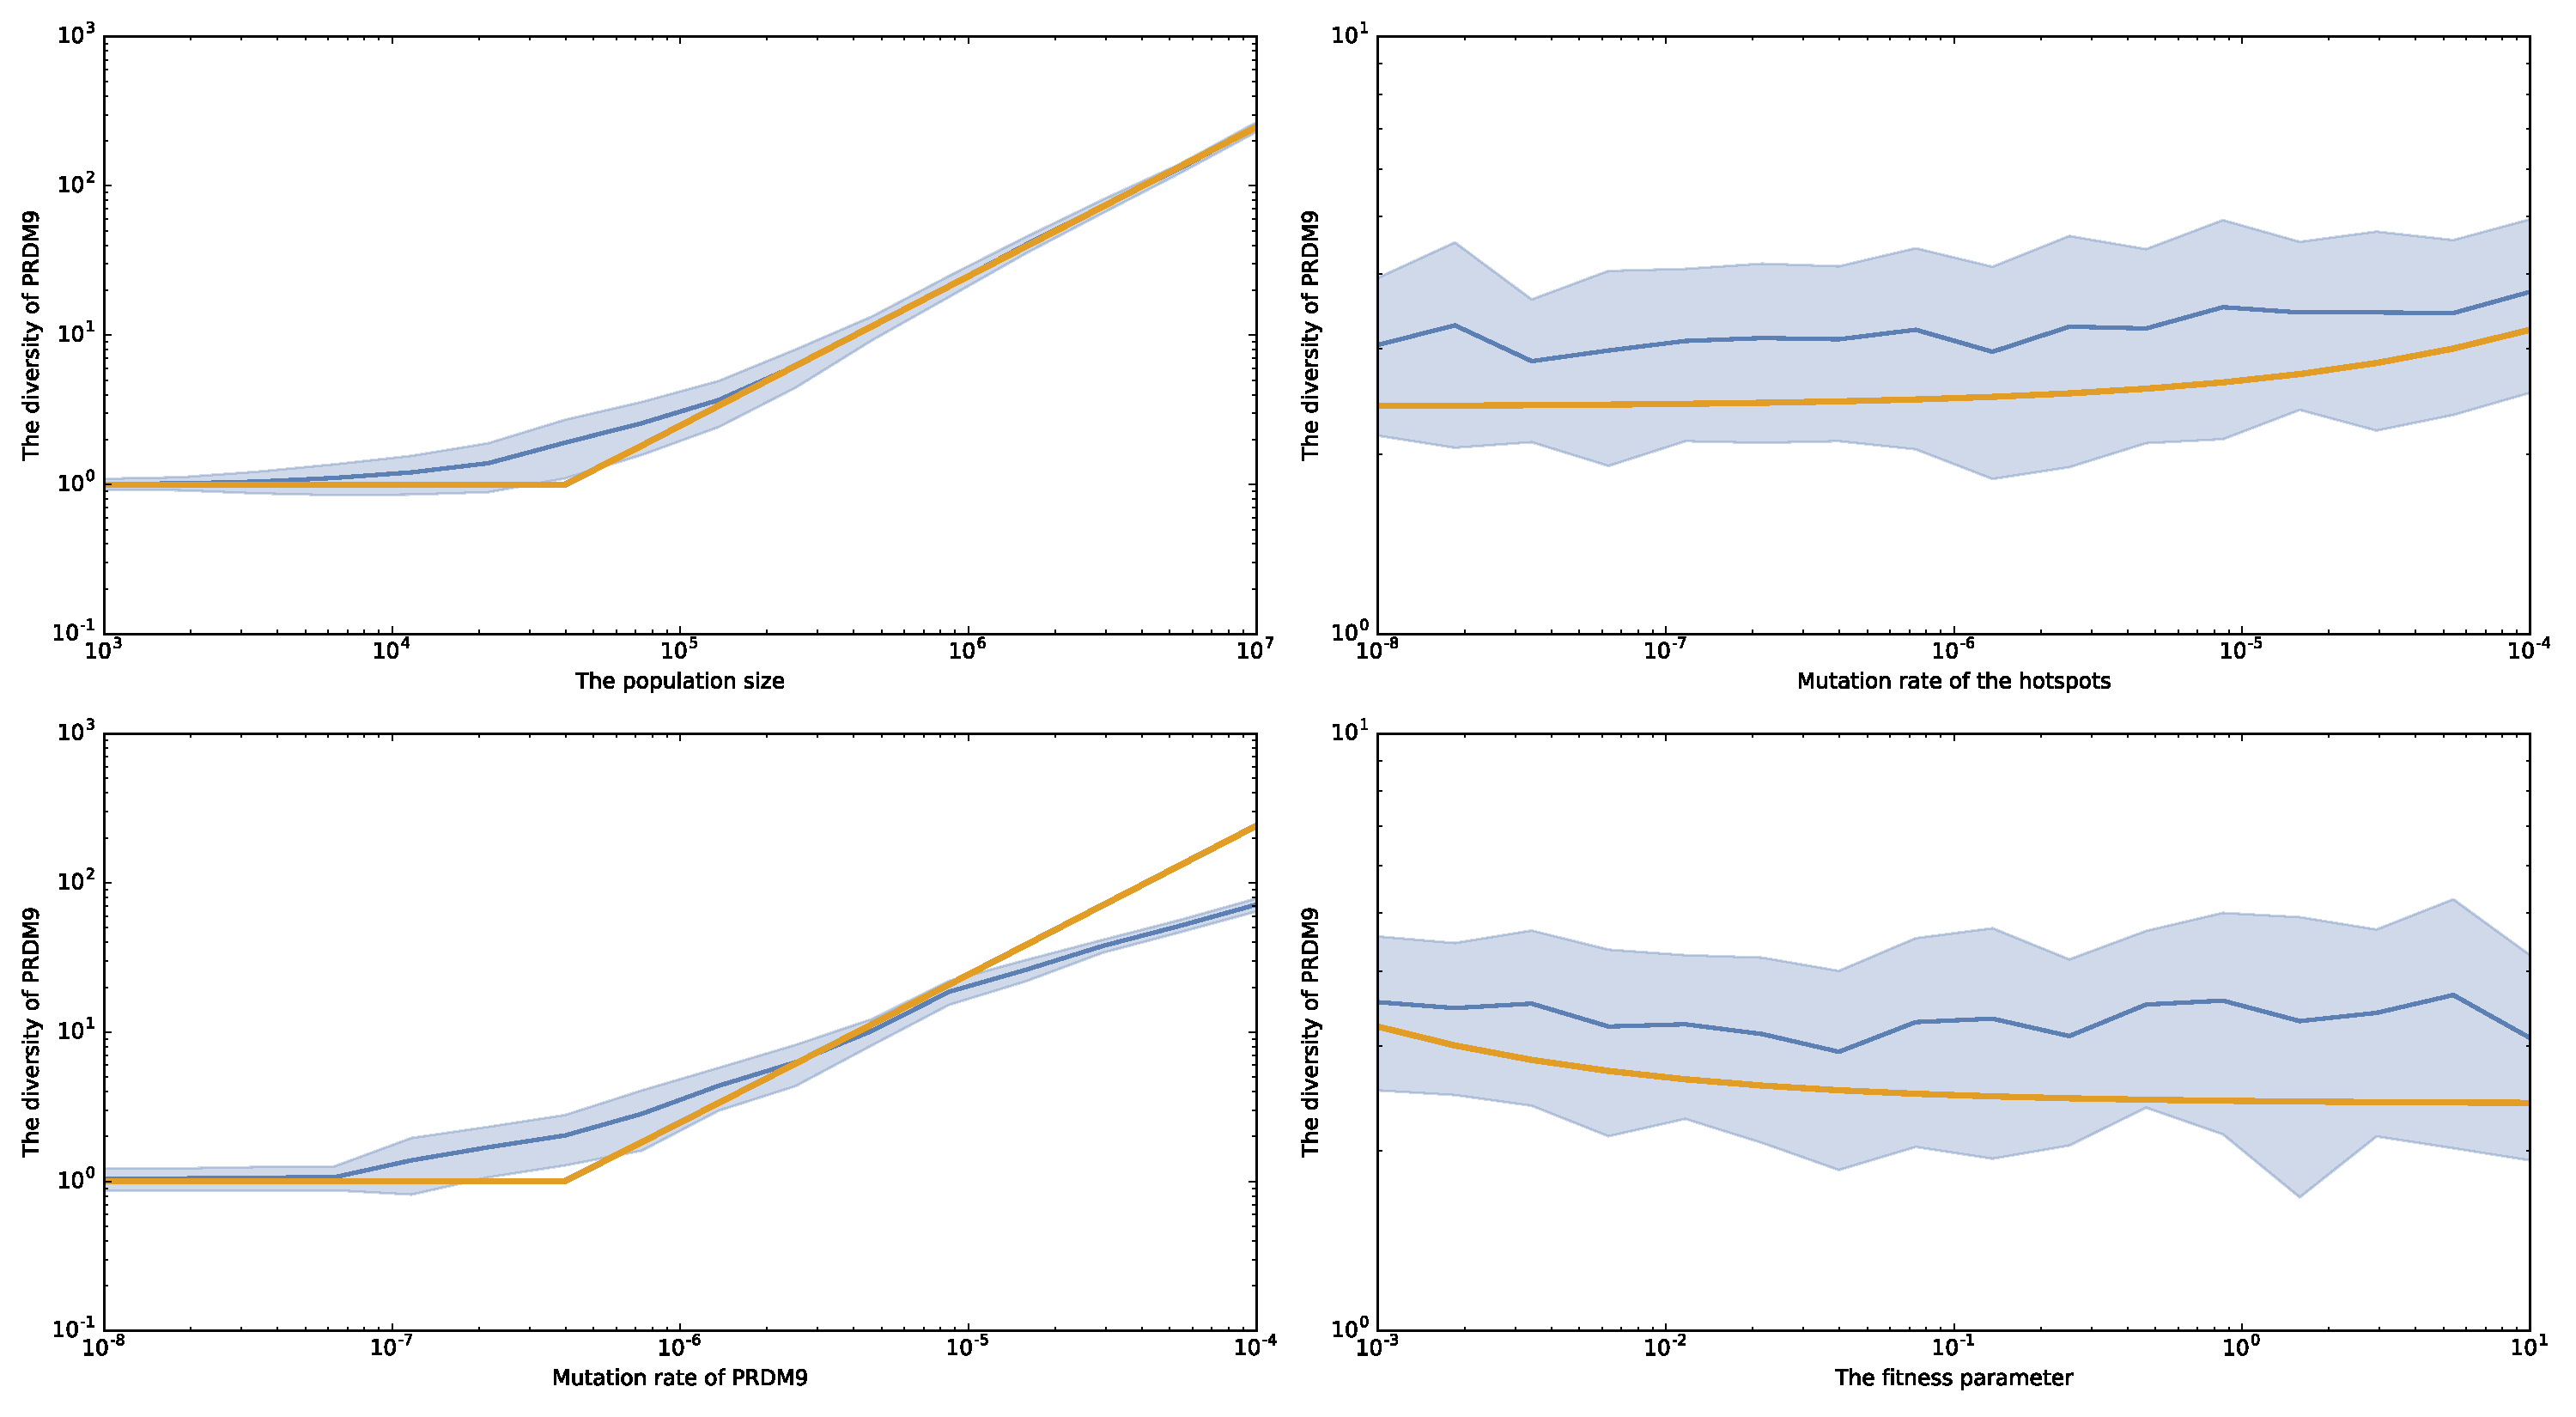
\includegraphics[width=0.8\textwidth]{Images/mean-field-prdm9-diversity.pdf}\\
		\caption{ \textbf{ Diversity.} 
}
\end{figure*}

\begin{figure*}[!ht]
	  \centering
       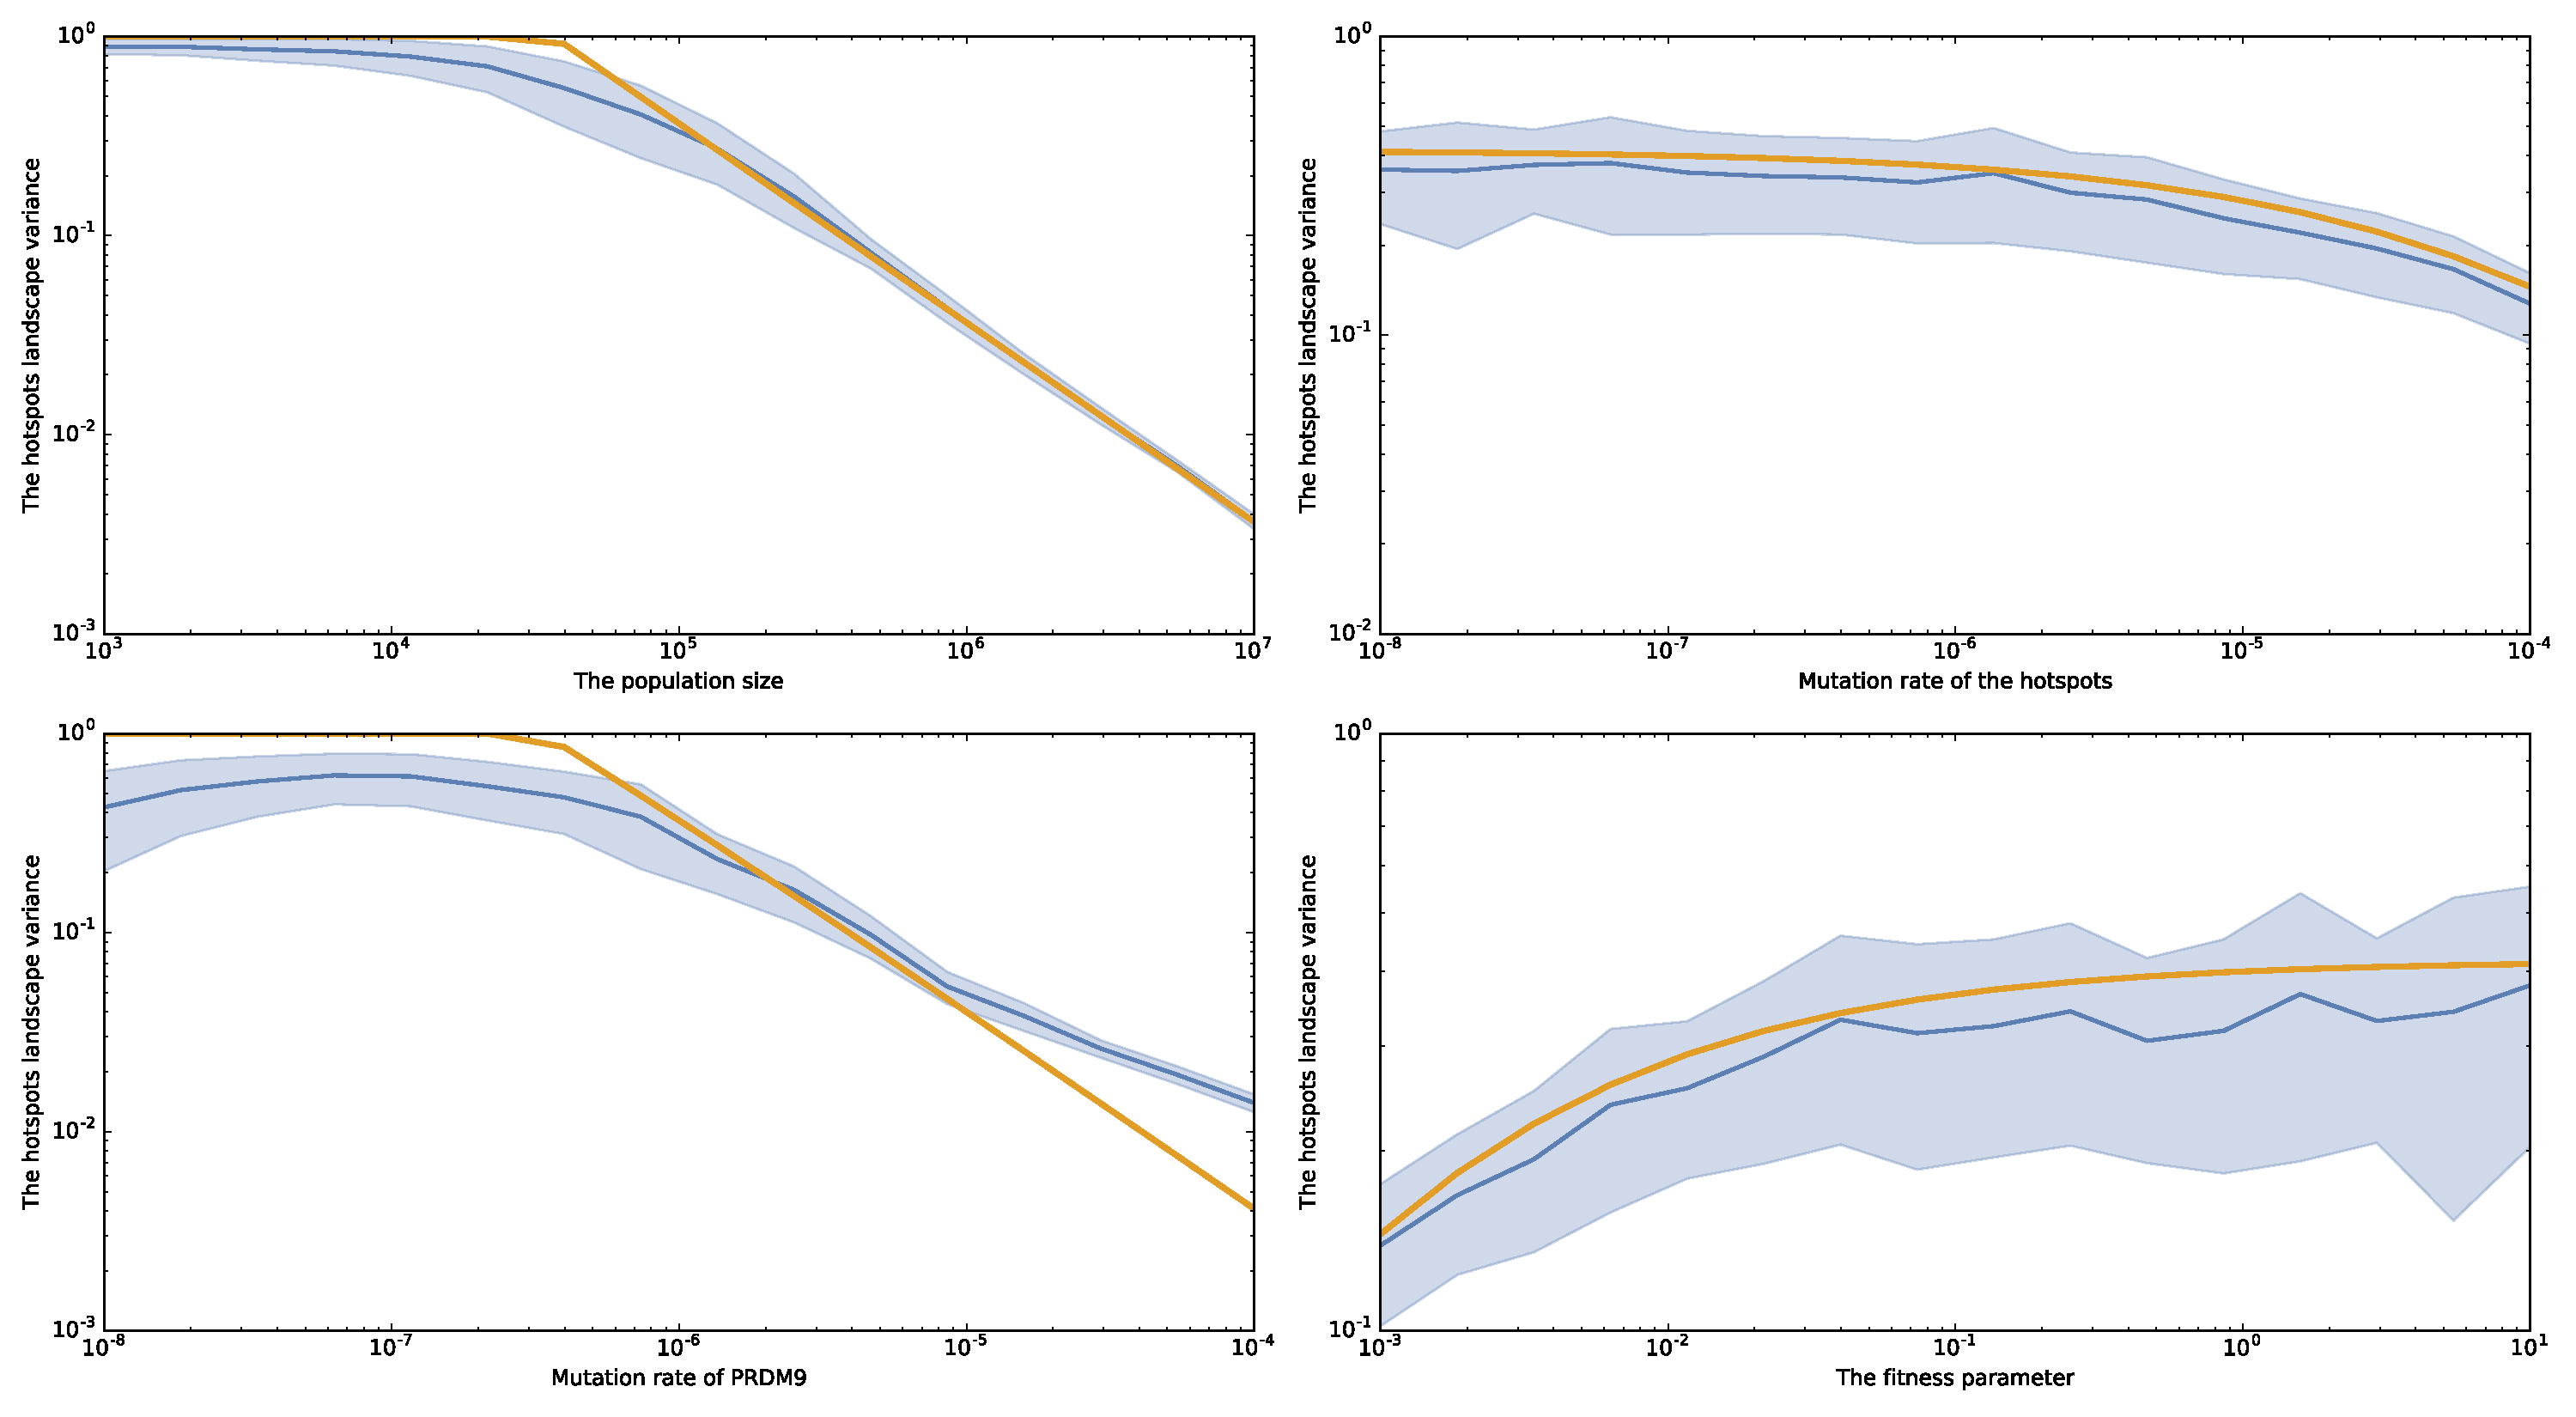
\includegraphics[width=0.8\textwidth]{Images/mean-field-landscape-variance.pdf}\\
		\caption{ \textbf{ Landscape of erosion.} 
}
\end{figure*}

\begin{figure*}[!ht]
	  \centering
       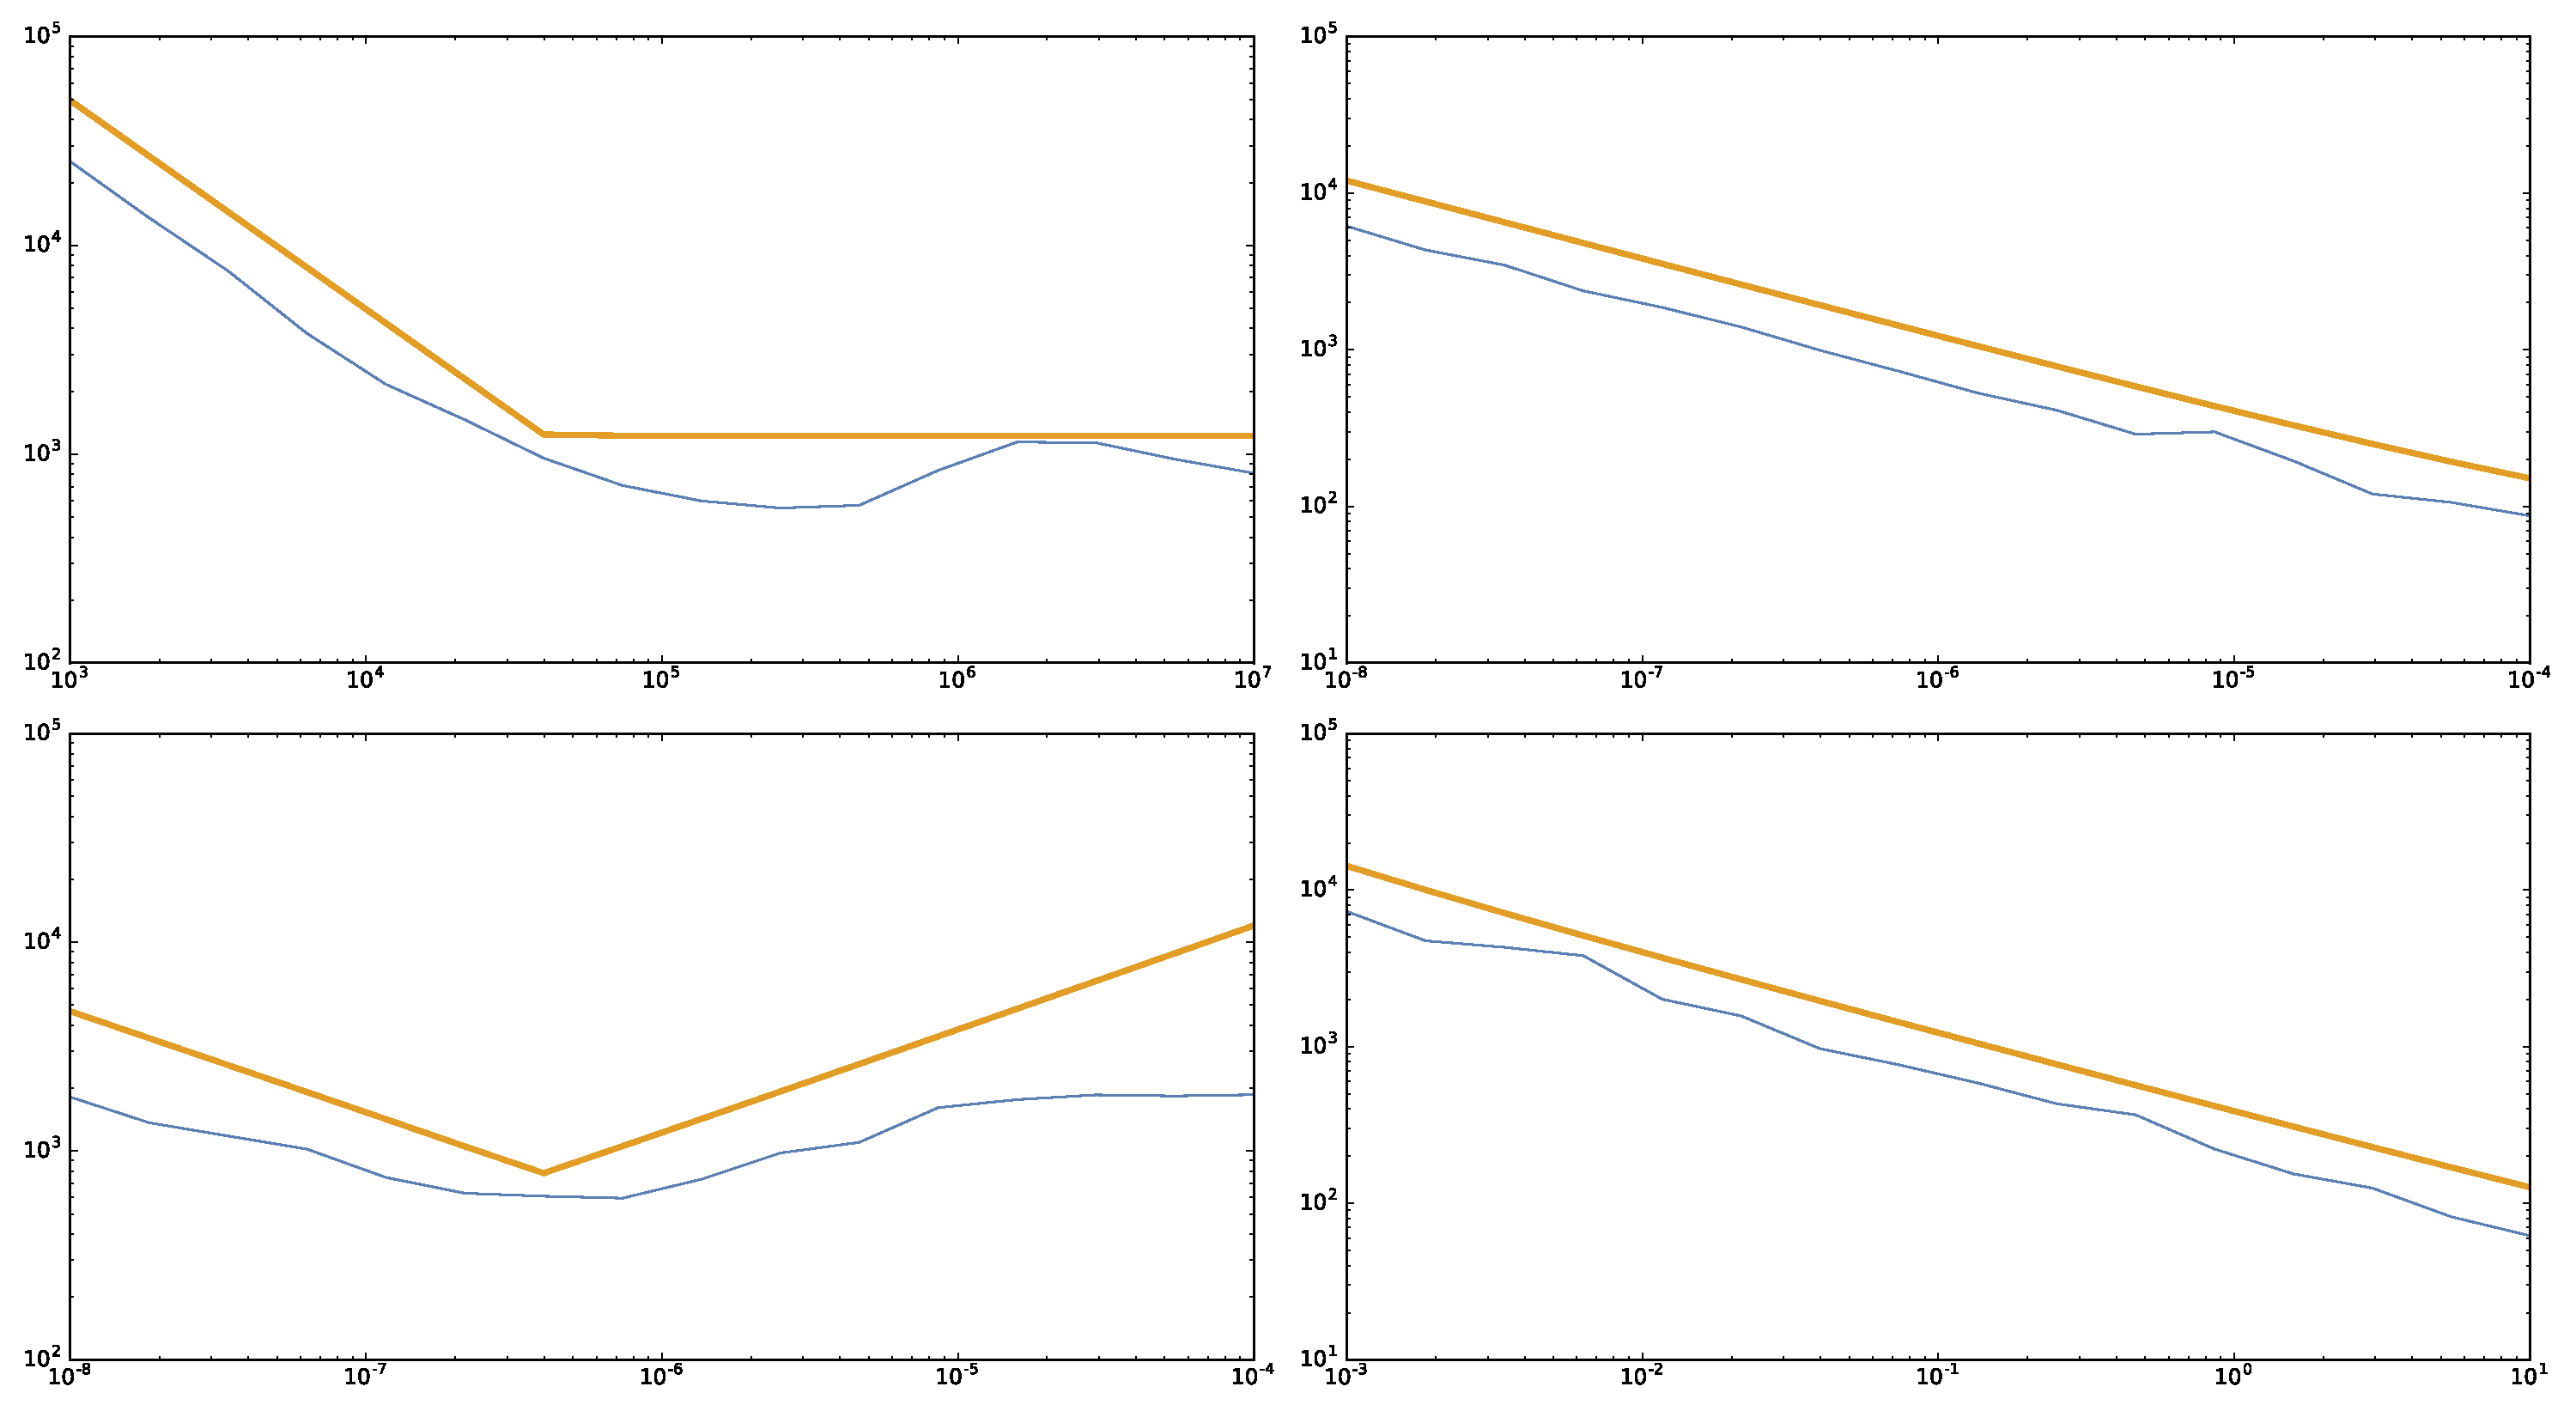
\includegraphics[width=0.8\textwidth]{Images/mean-field-turn-over.pdf}\\
		\caption{ \textbf{ Turn over time.} 
}
\end{figure*}

\clearpage

\section*{Small load estimation}
In solid yellow are the summary statistics estimated  from the parameters using small load development

\begin{figure*}[!ht]
	  \centering
       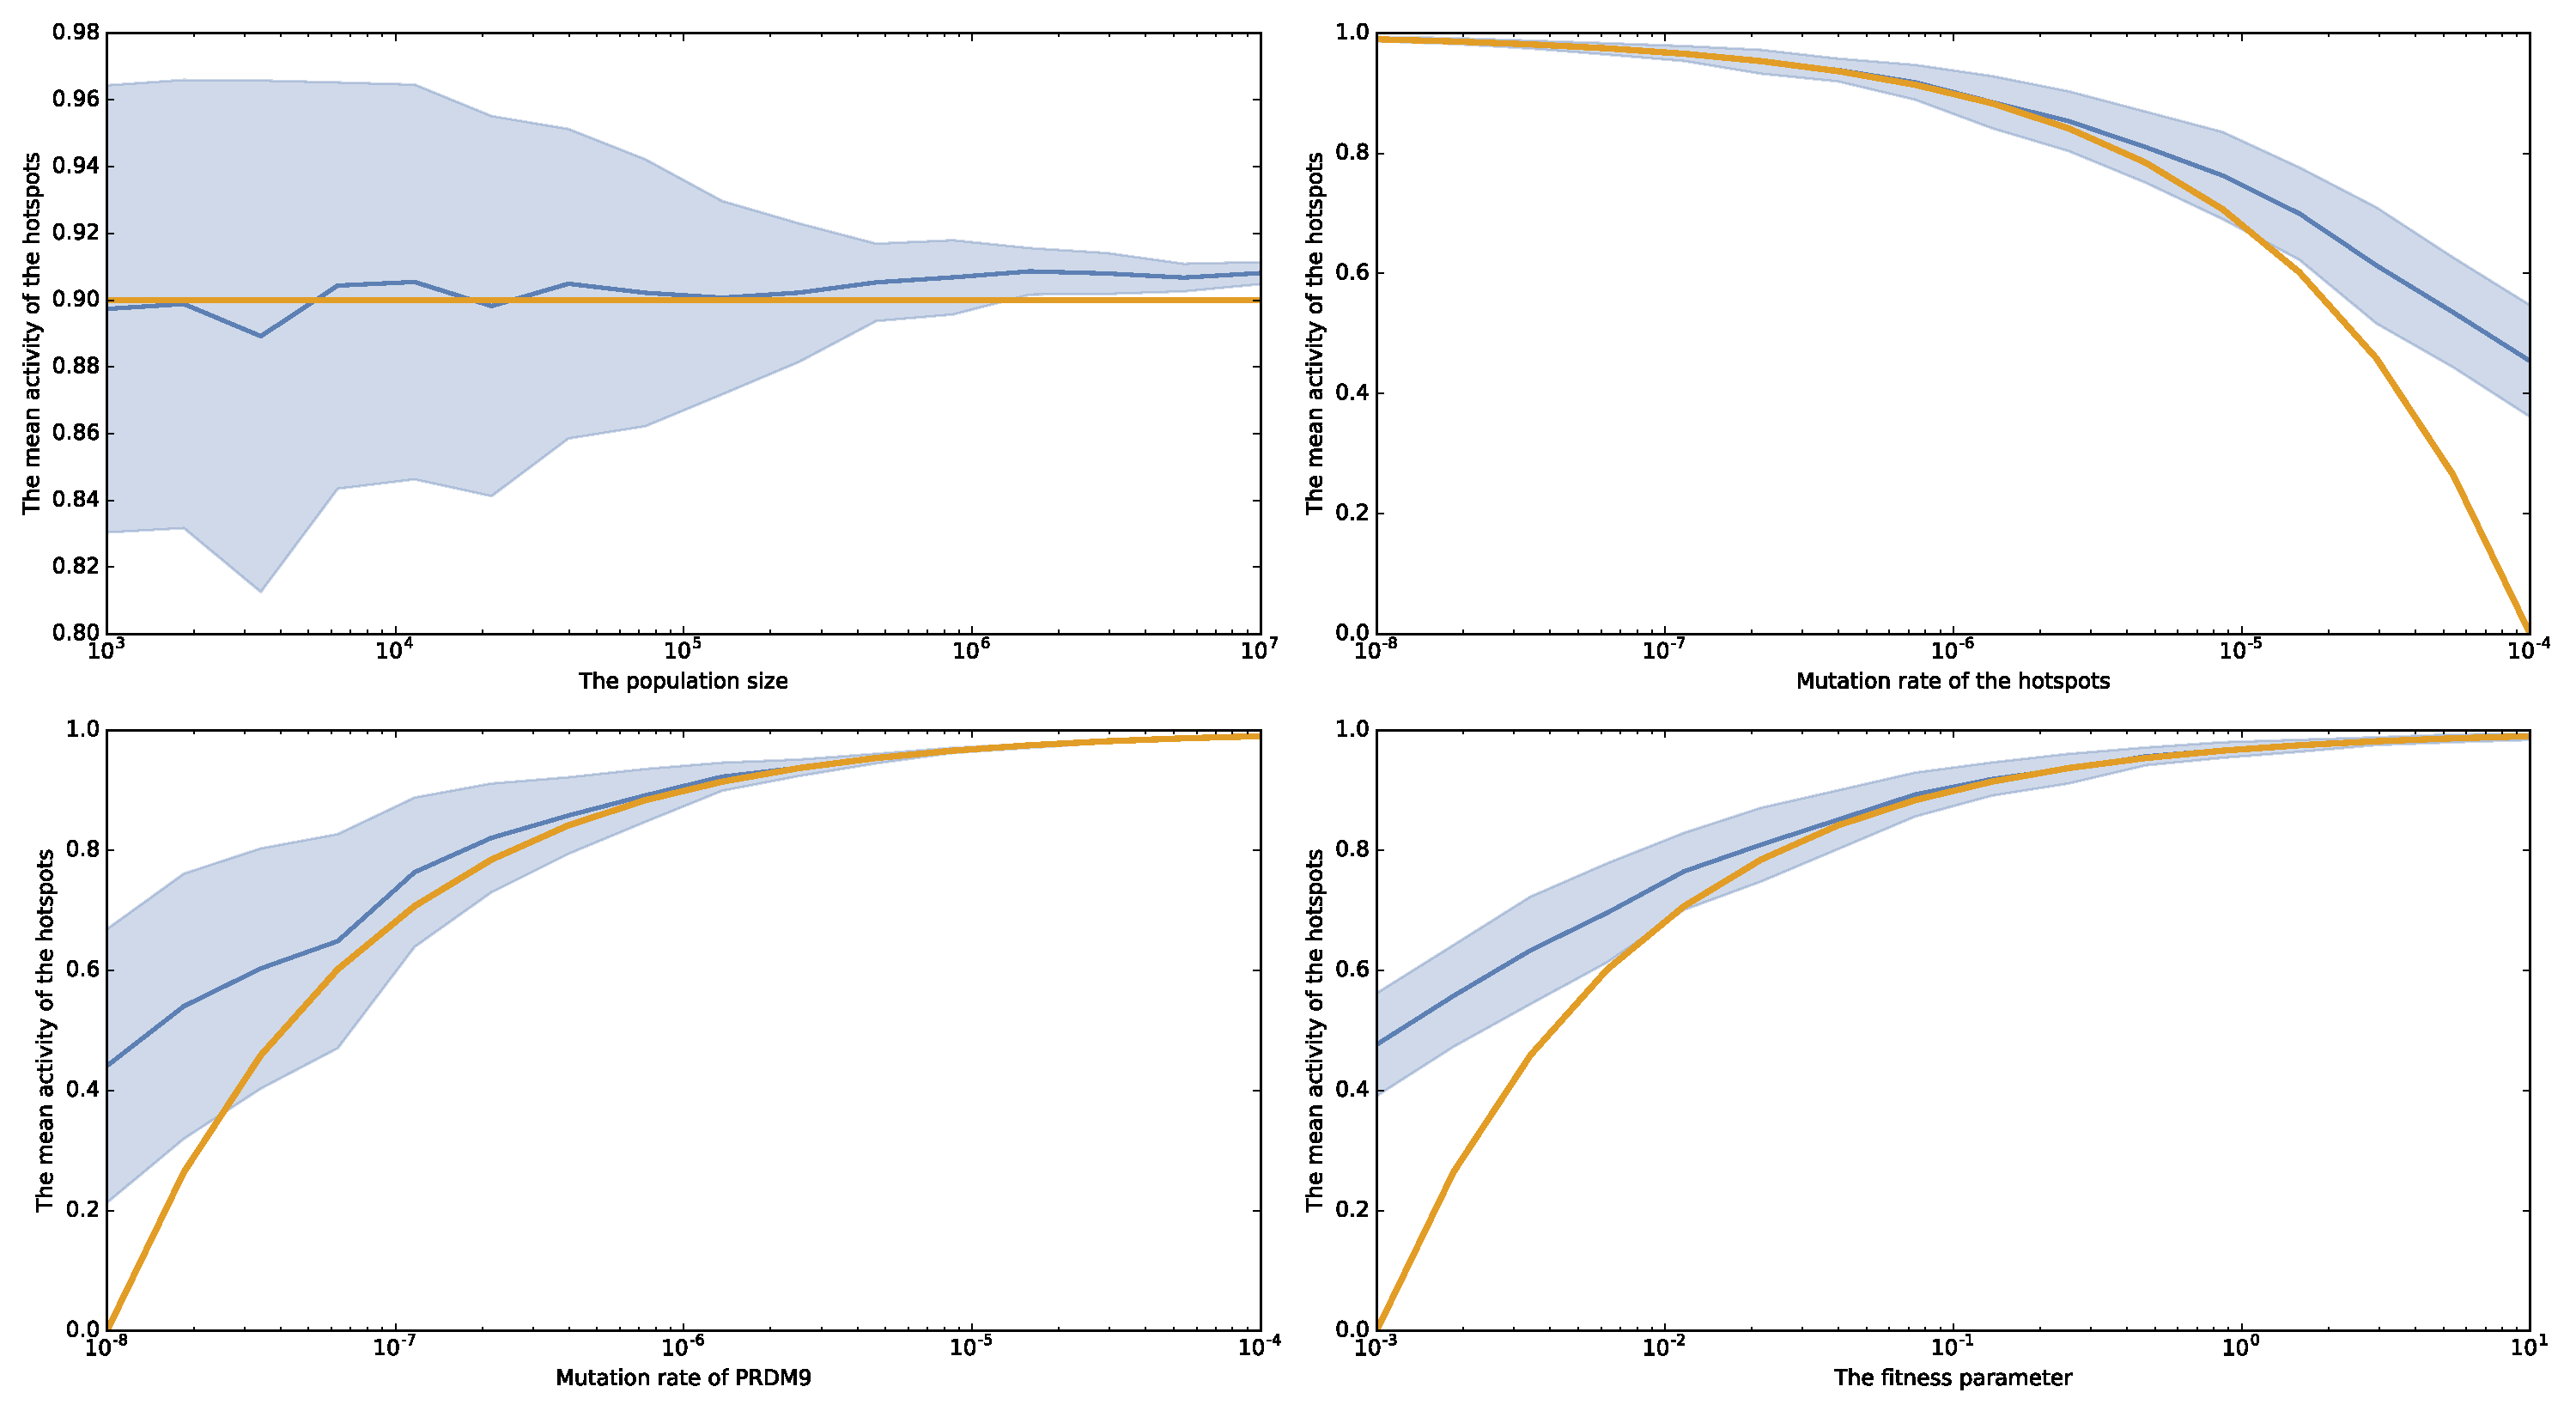
\includegraphics[width=0.8\textwidth]{Images/small-load-mean-activity.pdf}\\
		\caption{ \textbf{ Mean activity.} 
}
\end{figure*}

\begin{figure*}[!ht]
	  \centering
       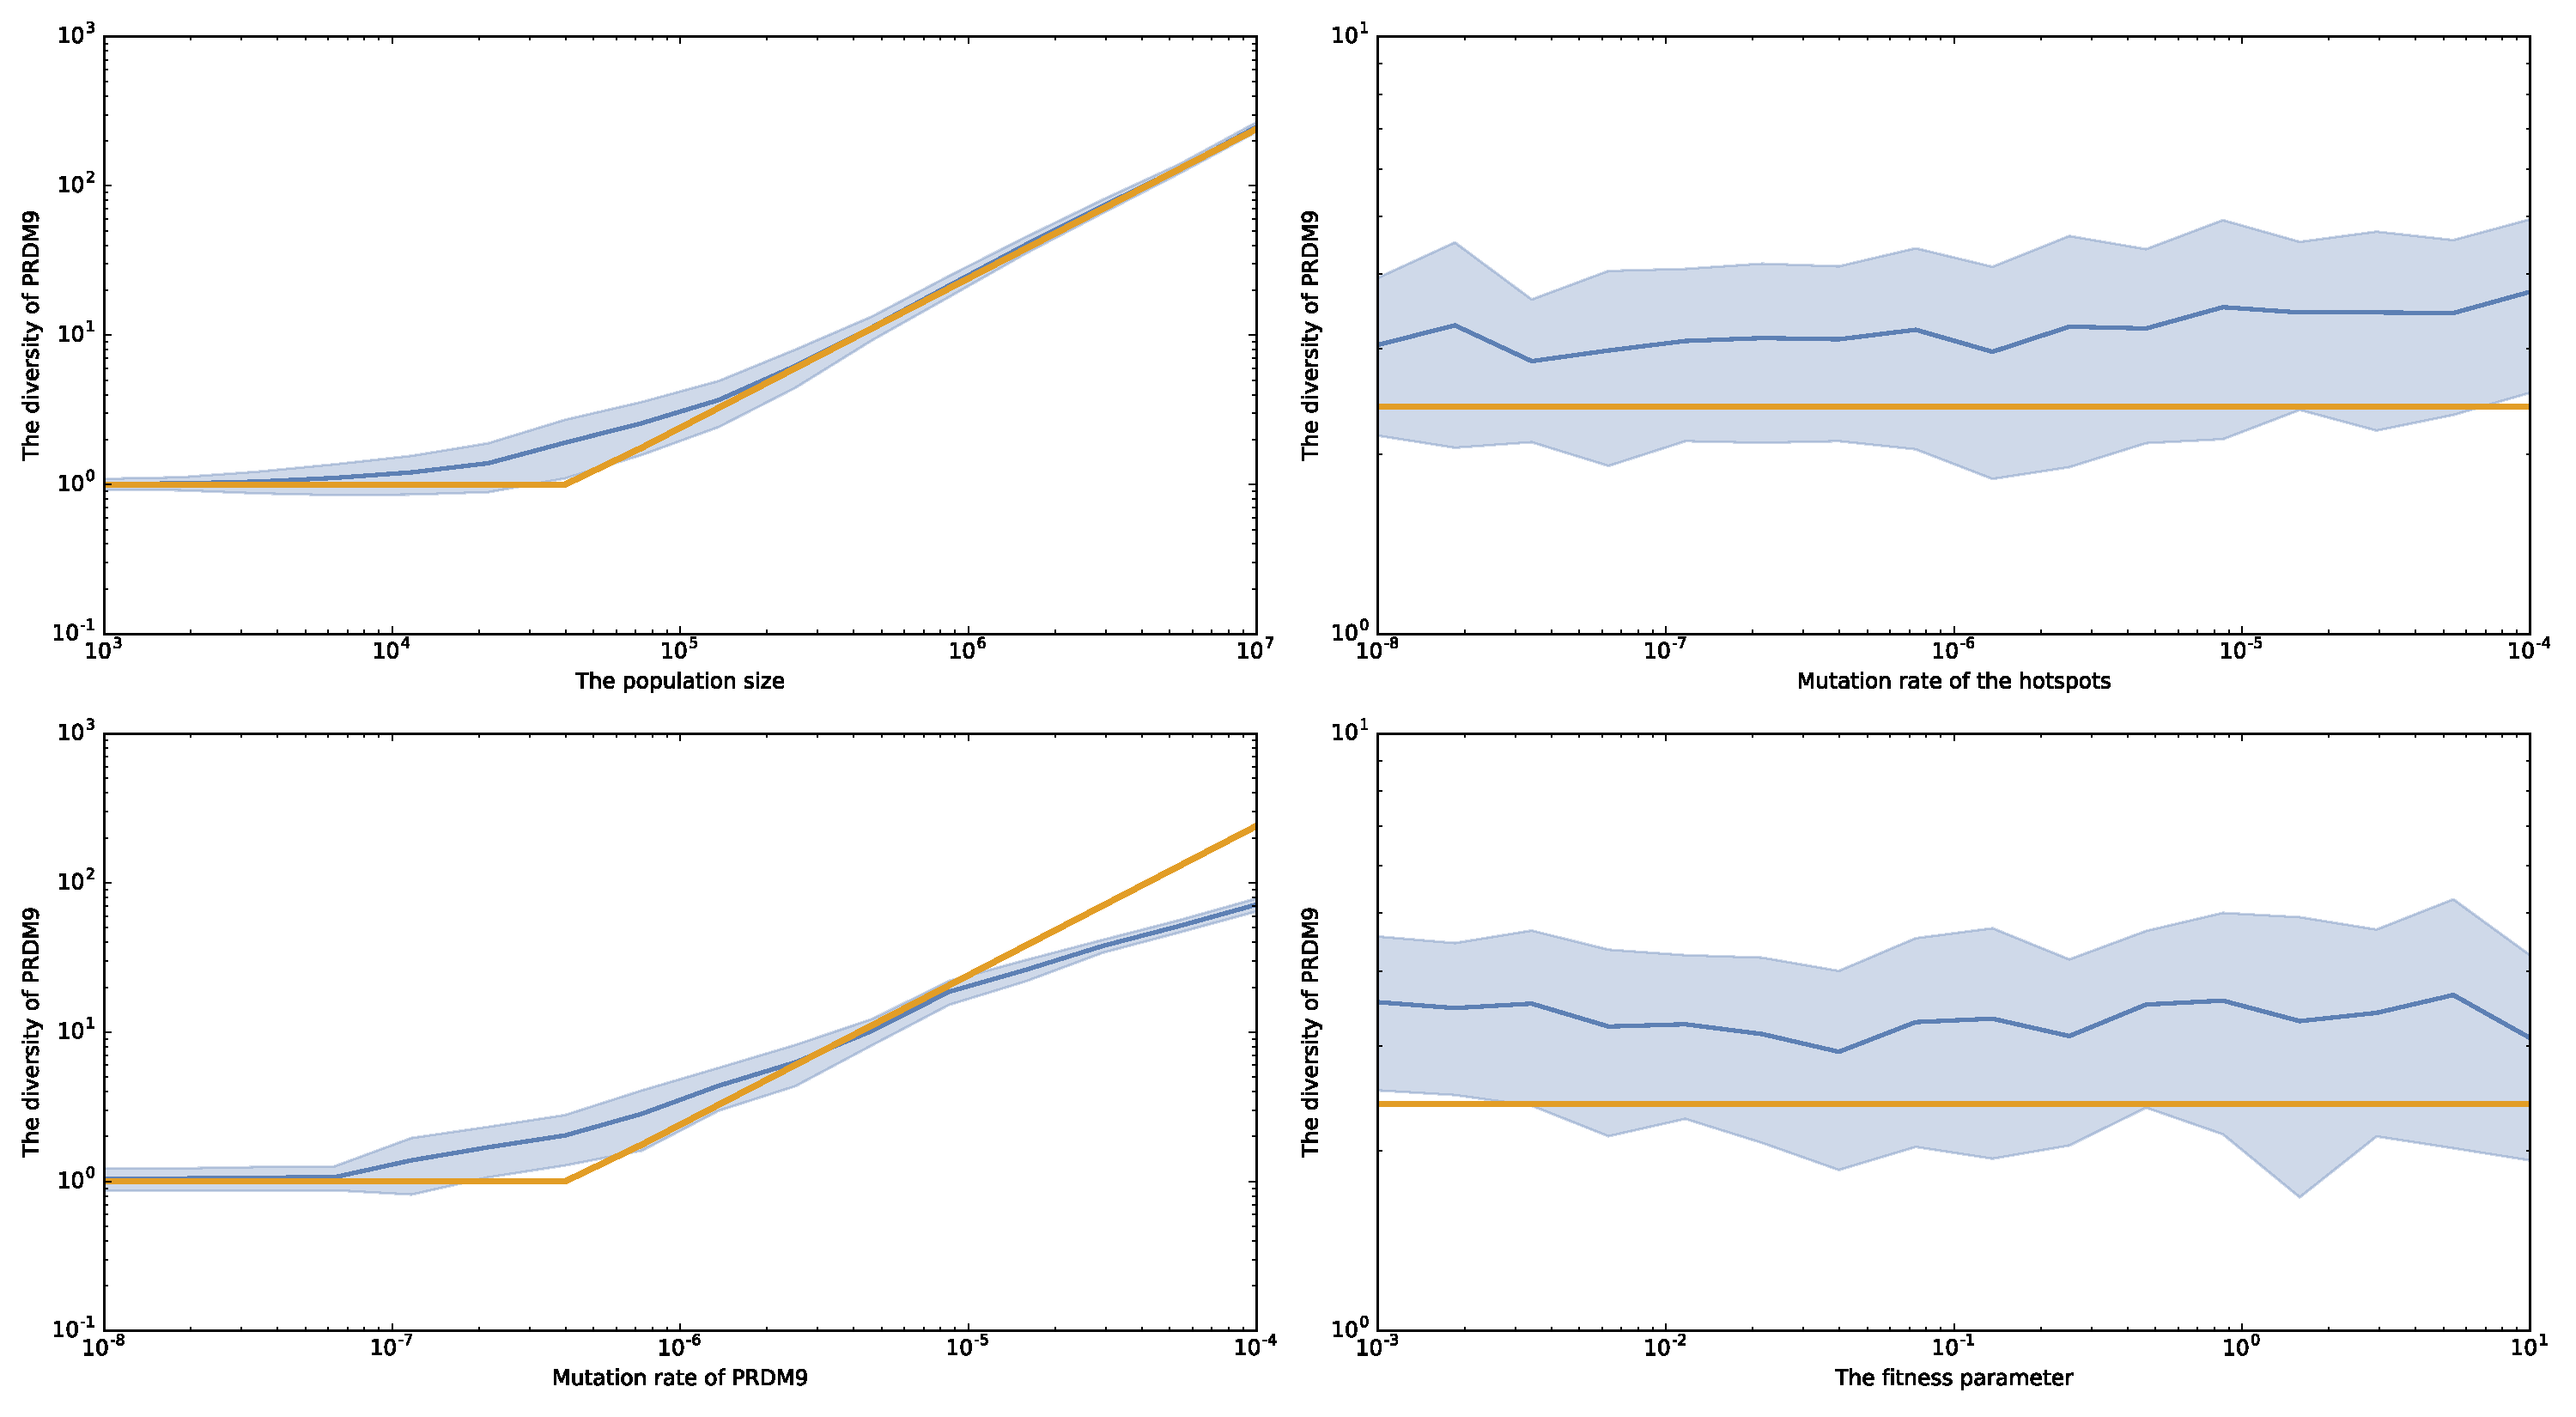
\includegraphics[width=0.8\textwidth]{Images/small-load-prdm9-diversity.pdf}\\
		\caption{ \textbf{ Diversity.} 
}
\end{figure*}

\begin{figure*}[!ht]
	  \centering
       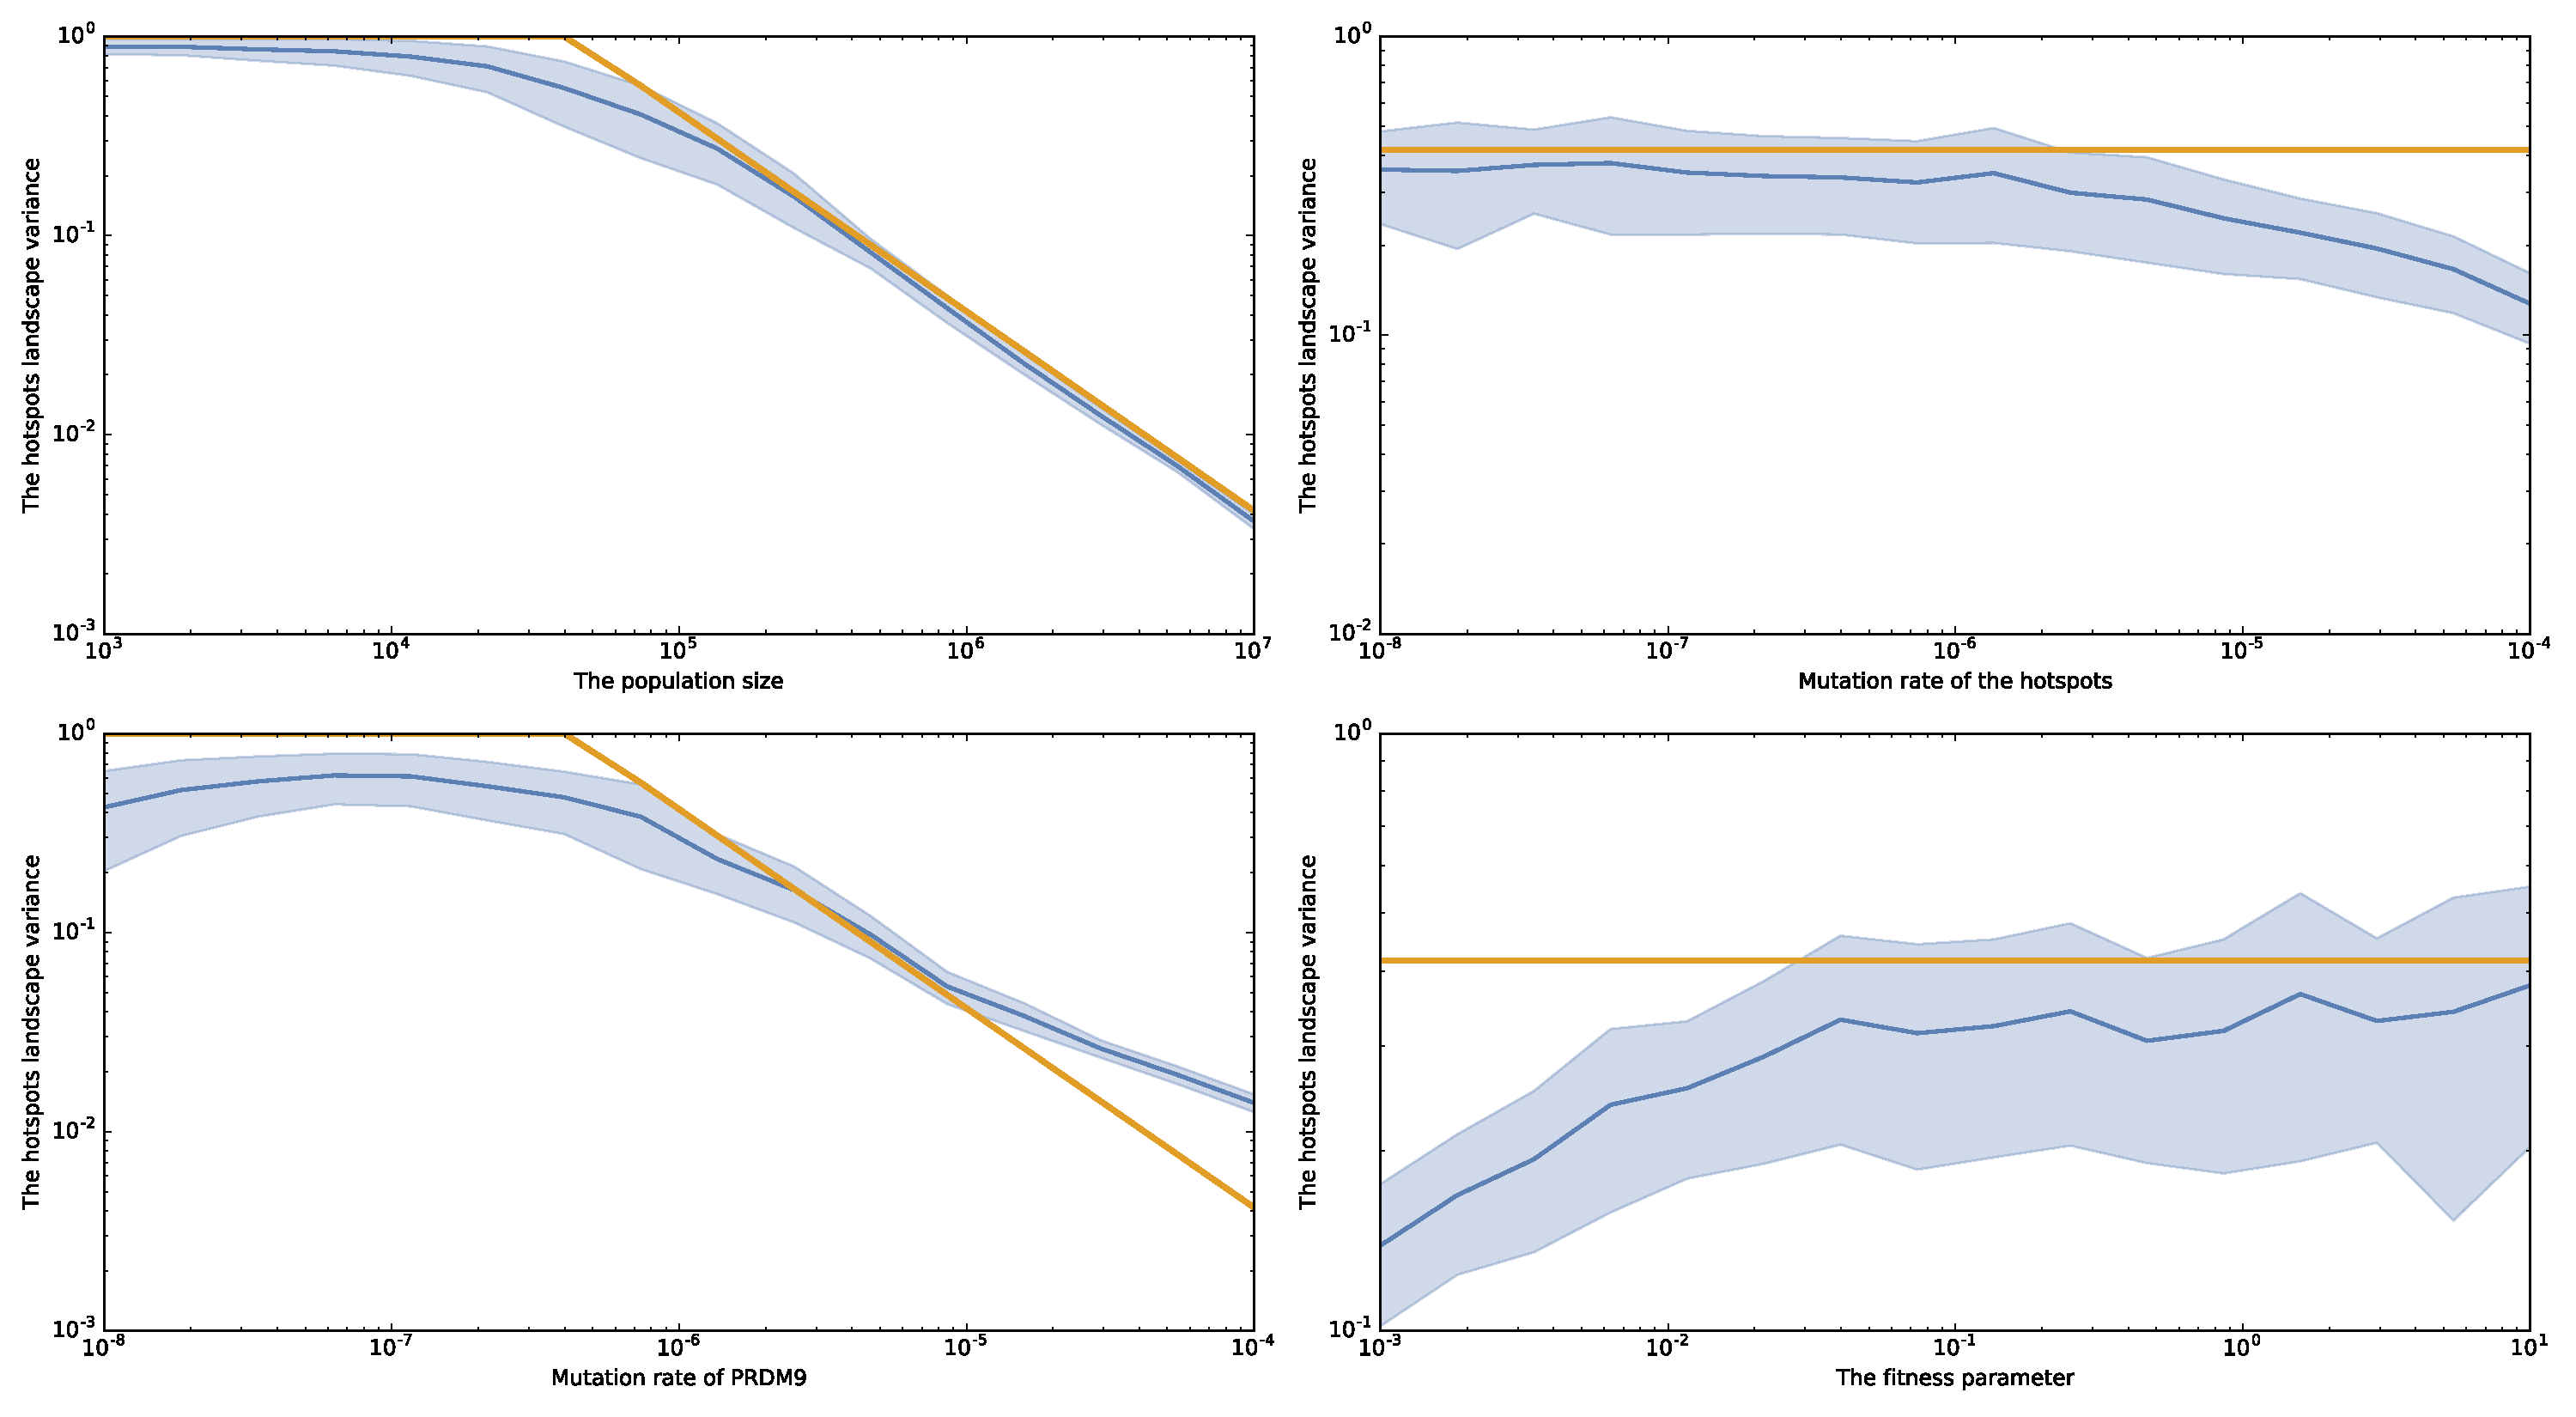
\includegraphics[width=0.8\textwidth]{Images/small-load-landscape-variance.pdf}\\
		\caption{ \textbf{ Landscape of erosion.} 
}
\end{figure*}

\begin{figure*}[!ht]
	  \centering
       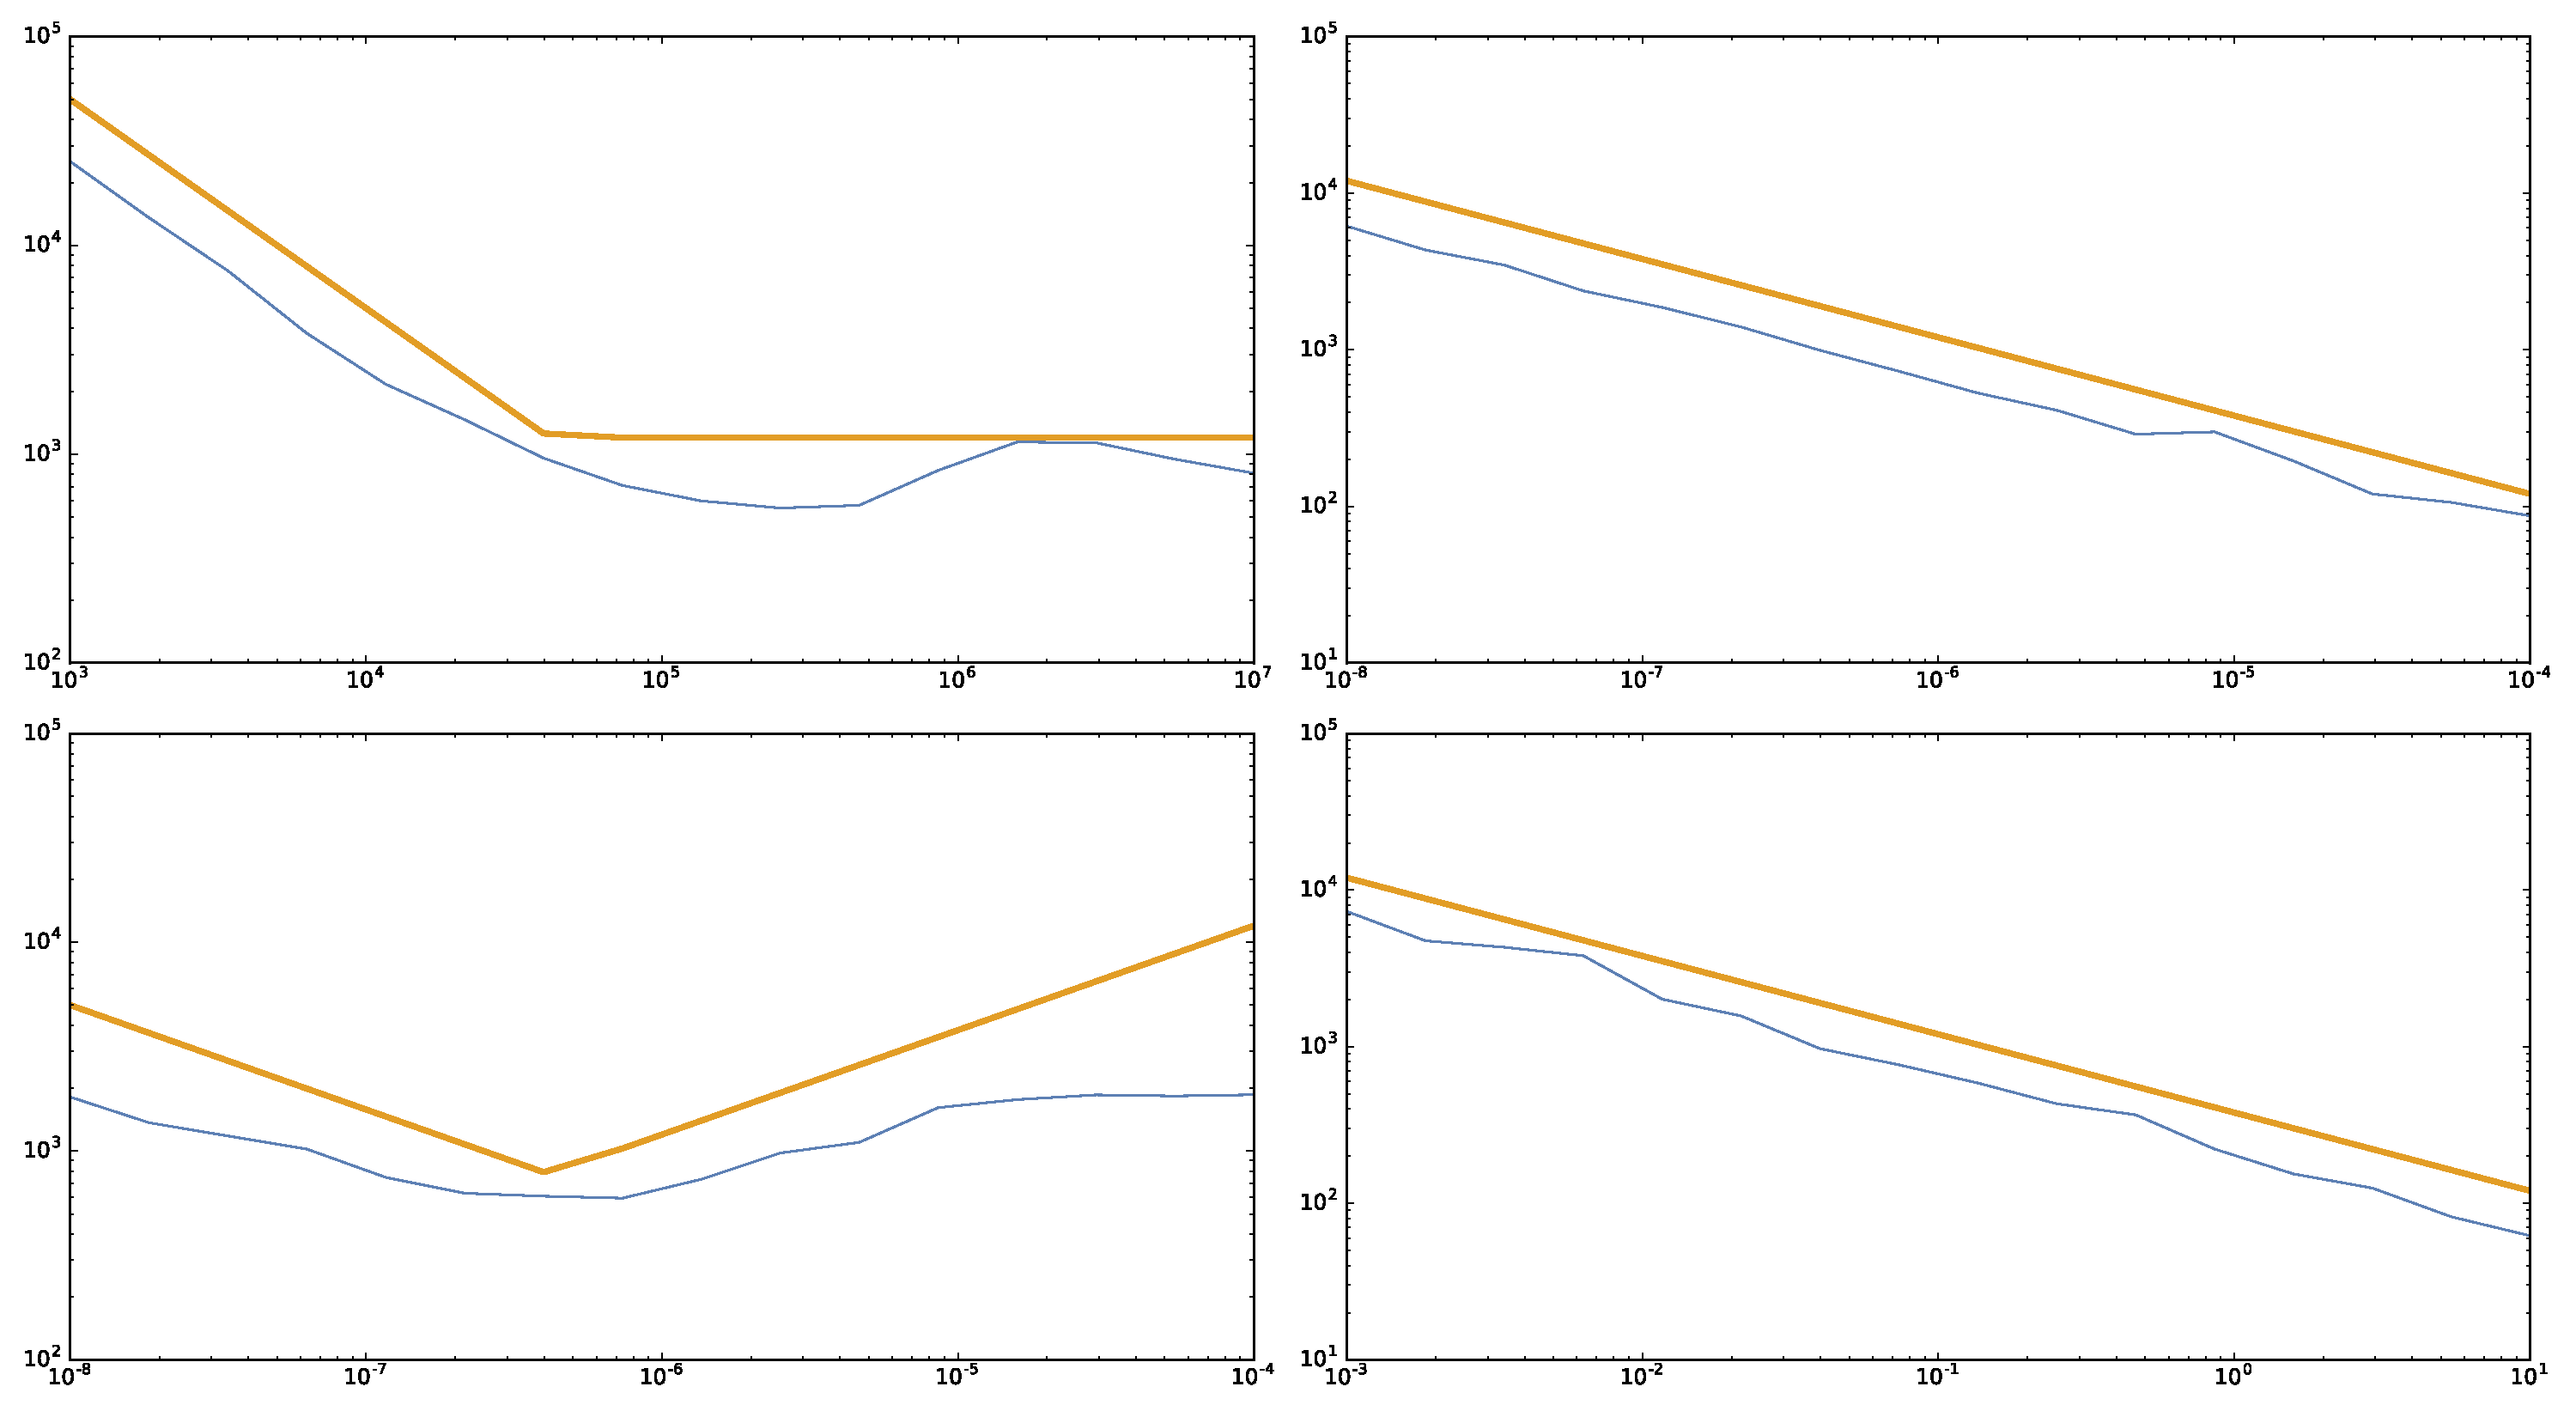
\includegraphics[width=0.8\textwidth]{Images/small-load-turn-over.pdf}\\
		\caption{ \textbf{ Turn over time.} 
}
\end{figure*}
\end{document}
